\documentclass[aspectratio=169]{beamer}

\title{Master's Thesis: Making offline handwriting editable}
\institute{Pattern Recognition Lab (CS~5)}
\date{September 9, 2019}
\author{Martin Stumpf}

\usetheme{fau-tf-lme}

% Sets the bib file
\usepackage[backend=biber, bibencoding=utf8, maxbibnames=99, % show all authors in the bibliography
			backref=false]{biblatex}
\addbibresource{presentation.bib}

%\newcommand{\comment}[1]{}

% MAGIC to remove citation numbers

\newcommand\footnotenonum[1]{%
  \begingroup
  \renewcommand\thefootnote{}\footnote{#1}%
  \addtocounter{footnote}{-1}%
  \endgroup
}

\makeatletter
\renewrobustcmd{\blx@mkbibfootnote}[2]{%
  \iftoggle{blx@footnote}
    {\blx@warning{Nested notes}%
     \addspace\mkbibparens{#2}}
    {\unspace
     \ifnum\blx@notetype=\tw@
       \expandafter\@firstoftwo
     \else
       \expandafter\@secondoftwo
     \fi
       {\csuse{blx@theendnote#1}{\protecting{\blxmkbibnote{end}{#2}}}}
       {\csuse{footnotenonum#1}{\protecting{\blxmkbibnote{foot}{#2}}}}}}
\makeatother





% Package subfig
\usepackage{subfig}
\usepackage{etoolbox}% http://ctan.org/pkg/etoolbox
\AtBeginEnvironment{figure}{\setcounter{subfigure}{0}}% Resets subfigure counter at start of figure environment

% mathstuff
\usepackage{amsmath,amssymb}
\usepackage{mathtools}
\DeclarePairedDelimiter{\norm}{\lVert}{\rVert}
\usepackage{bm}


\usepackage{booktabs}
\usepackage{graphics}

\begin{document}

\maketitle
  
  
  
  
\begin{frame}
  \tableofcontents
\end{frame}




\section{Introduction}

\begin{frame}{Introduction}
\textbf{"Making offline handwriting editable"}

\begin{itemize}
\item offline vs online handwriting:\\
\begin{columns}
\column{0.27\textwidth}
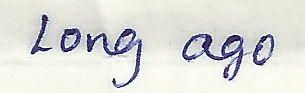
\includegraphics[scale=2.0]{../initial_presentation/pics/12th-std1-crop.png}
%\hspace{15pt}
\column{0.45\textwidth}
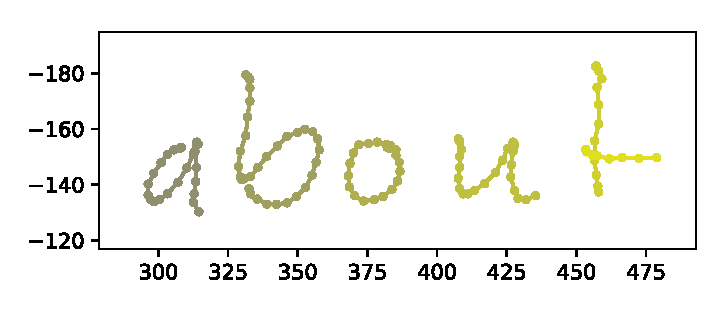
\includegraphics[scale=0.4]{../initial_presentation/pics/PenPositionsImages.pdf}
\end{columns}\vspace{5pt}
\item `editable':\\
\vspace{1em}
\hspace{0.7em}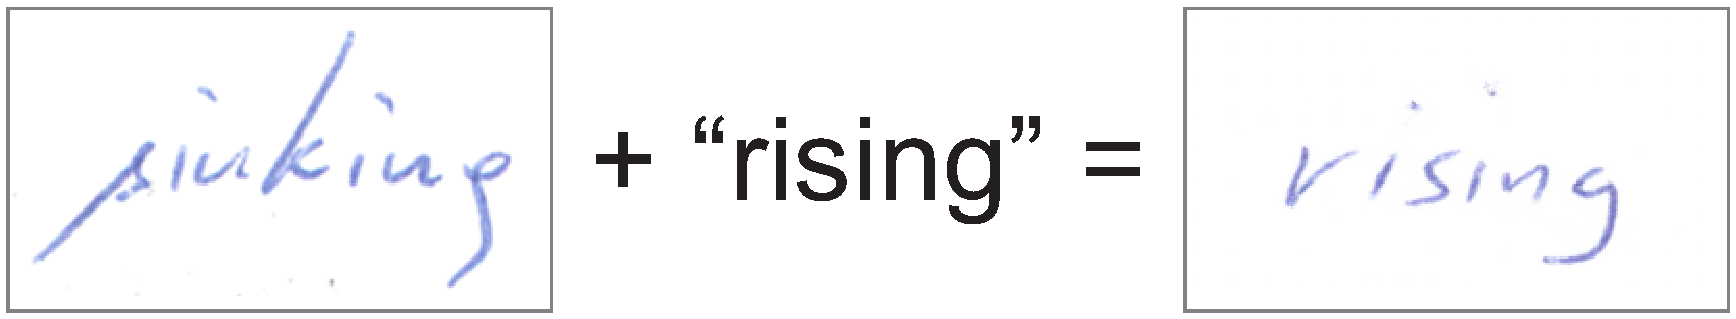
\includegraphics[width=0.5\textwidth]{assets/editable_explanation.pdf}
\end{itemize}
\end{frame}



\begin{frame}{General Approach}
\textbf{Goal:}
\begin{itemize}
\item Full offline-to-offline handwriting style transfer algorithm
\end{itemize}
\vspace{1em}

\textbf{Related Work:}
\begin{itemize}
\item \emph{Alex Graves}: "Generating Sequences With Recurrent Neural Networks" (2013)
\item \emph{Aksan et al.}: "DeepWriting: Making Digital Ink Editable via Deep Generative Modeling" (2018)
\item Disadvantage: online data, no pen or background style
\end{itemize}
\vspace{1em}

\textbf{Idea:}
\begin{itemize}
\item Conversion of offline to online handwriting
\item Usage of existing online handwriting synthesis algorithm
\item Additional style transfer for pen style and background
\end{itemize}

\end{frame}




\begin{frame}{Goals}
%\textbf{Goals of this thesis:}
\begin{itemize}
\item Full offline-to-offline handwriting style transfer algorithm
\item Finding a robust algorithm for handwriting skeletonization
\item Is an offline to online handwriting conversion sufficient to use online algorithms?
\item Finding a way to transfer the pen style to the output image
\item \emph{Optional:} Finding a way to transfer the background style to the output image
\end{itemize}
\end{frame}




\section{Pipeline Overview}
\begin{frame}{Pipeline Overview}
\begin{center}
\vspace{-1em}
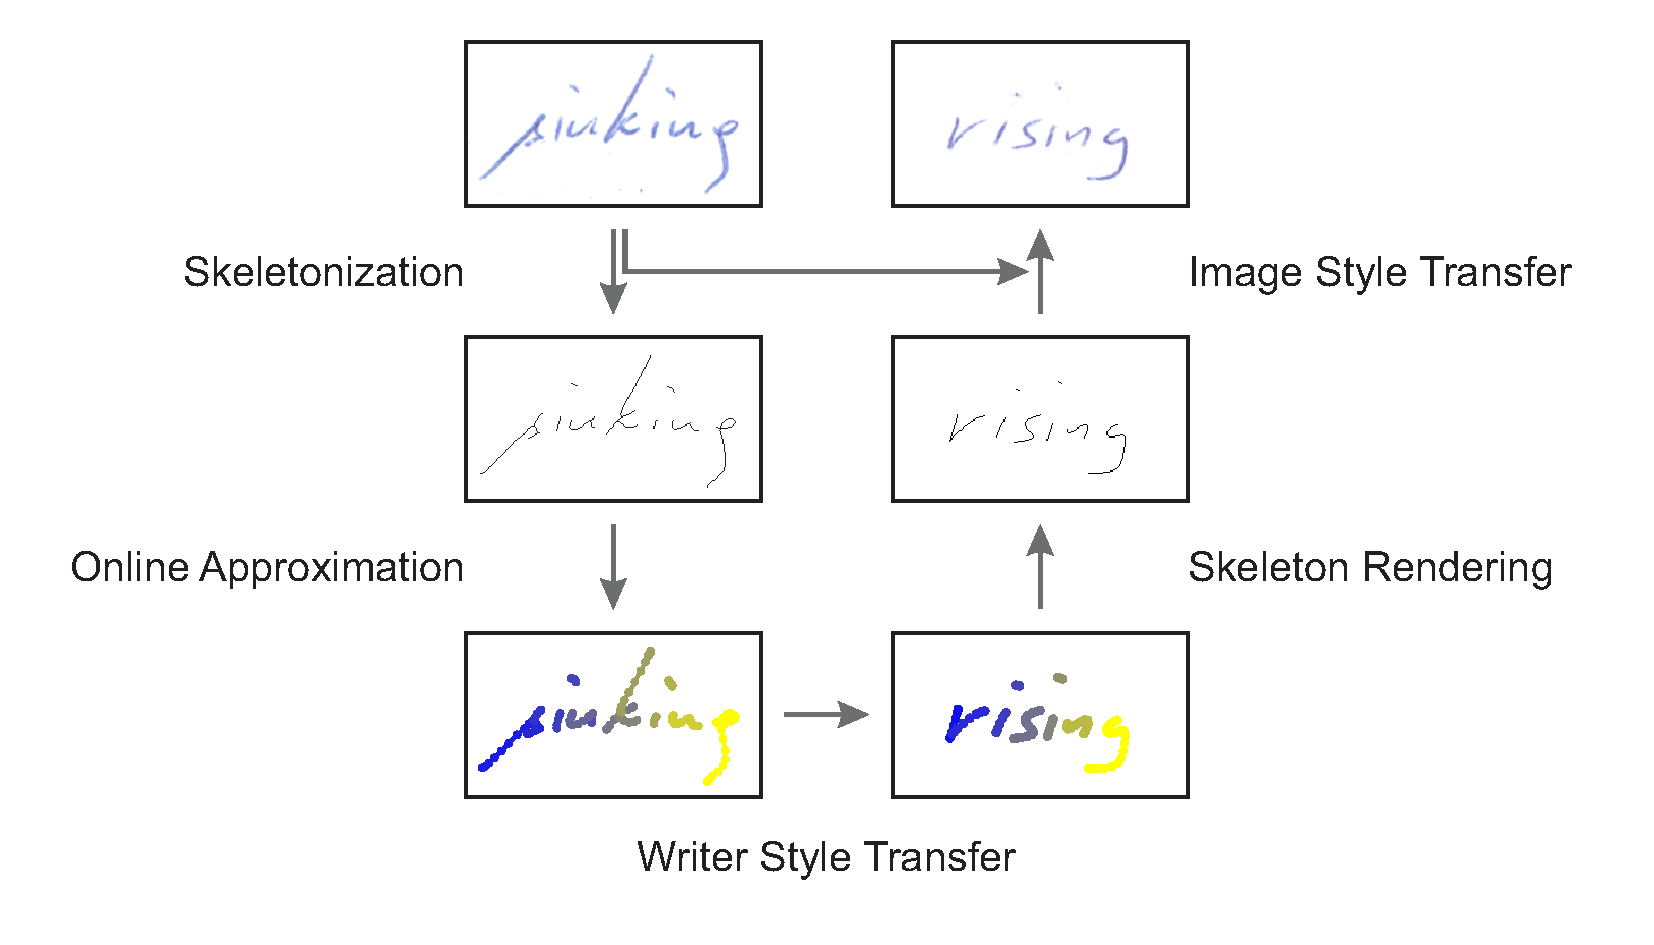
\includegraphics[width=0.85\textwidth]{../thesis/assets/pipeline.pdf}
\end{center}
\end{frame}



\section{Stage 1: Skeletonization}
\begin{frame}{Skeletonization}
\begin{center}
\vspace{-1em}
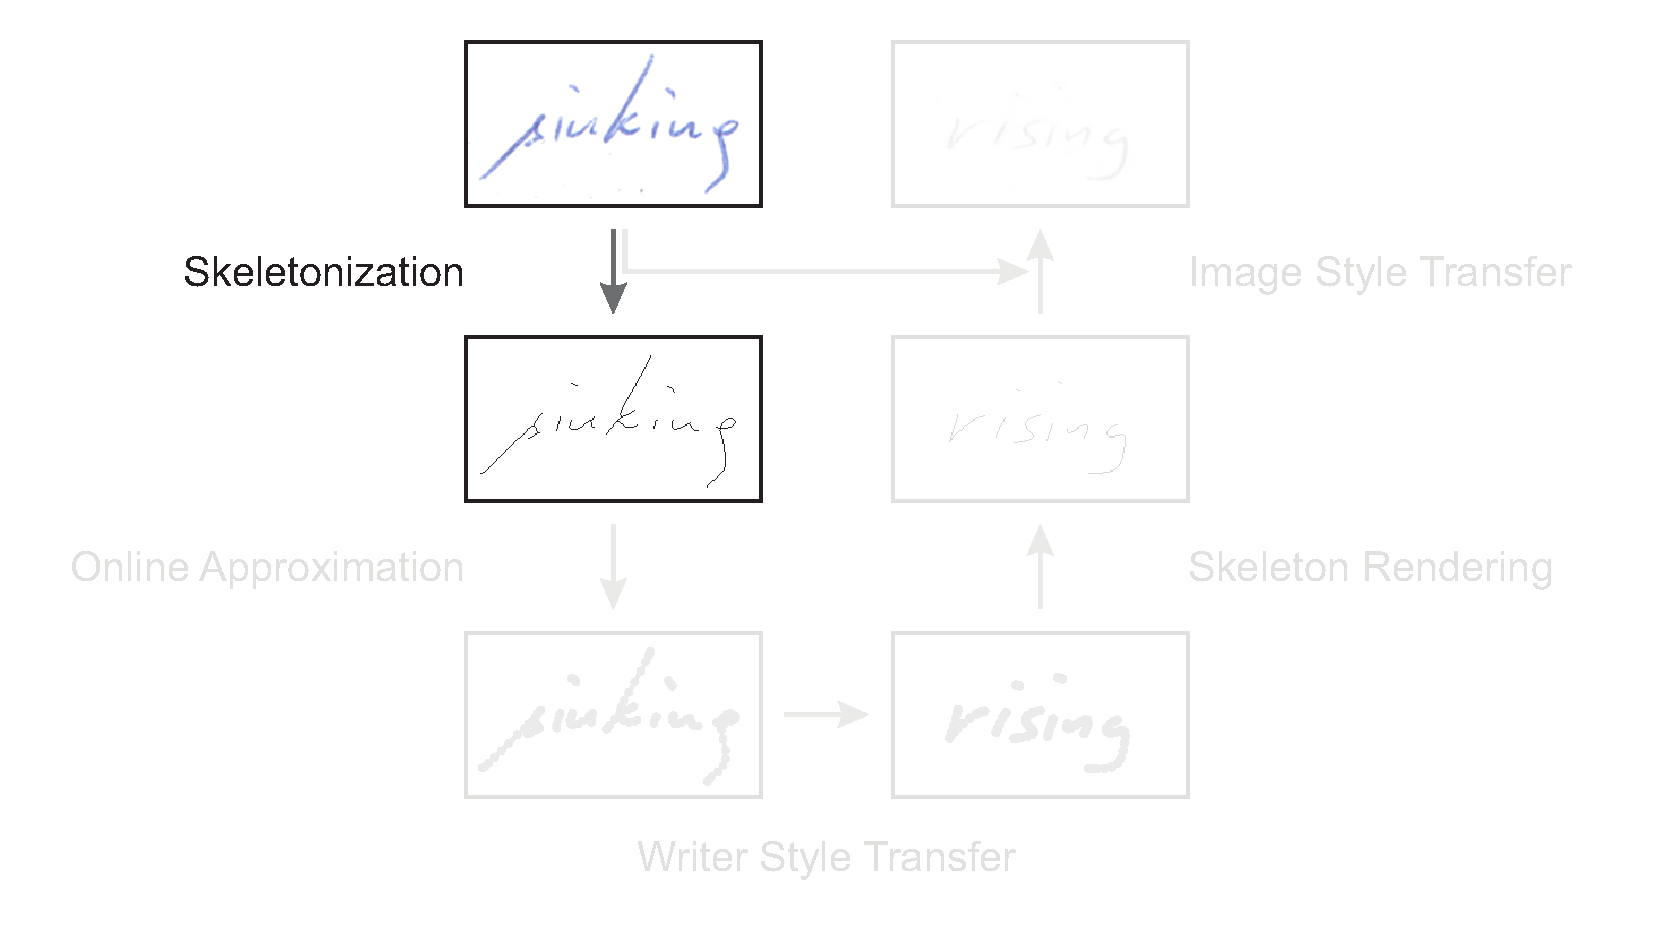
\includegraphics[width=0.85\textwidth]{assets/pipeline/pipeline_skeletonization.pdf}
\end{center}
\end{frame}



\begin{frame}{Background - Pix2Pix (2016, Phillip Isola et al.)}
\vspace{-1em}
\begin{center}
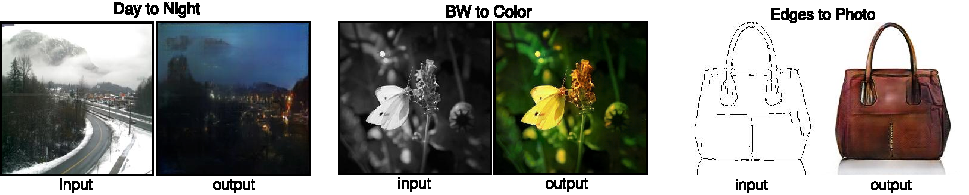
\includegraphics[width=0.95\textwidth]{assets/pix2pix_examples_small.pdf}
\end{center}
%\vspace{-1em}
\textbf{Capabilities:}
\begin{itemize}
\item mapping from one visual representation to another
\end{itemize}
\textbf{Requirements:}
\begin{itemize}
\item pairwise annotations in training dataset
\end{itemize}
\footfullcite{pix2pix}
\end{frame}



\begin{frame}{Background - Pix2Pix (2016, Phillip Isola et al.)}
\vspace{-1em}
\textbf{Innovations of Pix2Pix}
\vspace{1em}
\begin{itemize}
\item U-Net\\
\begin{center}
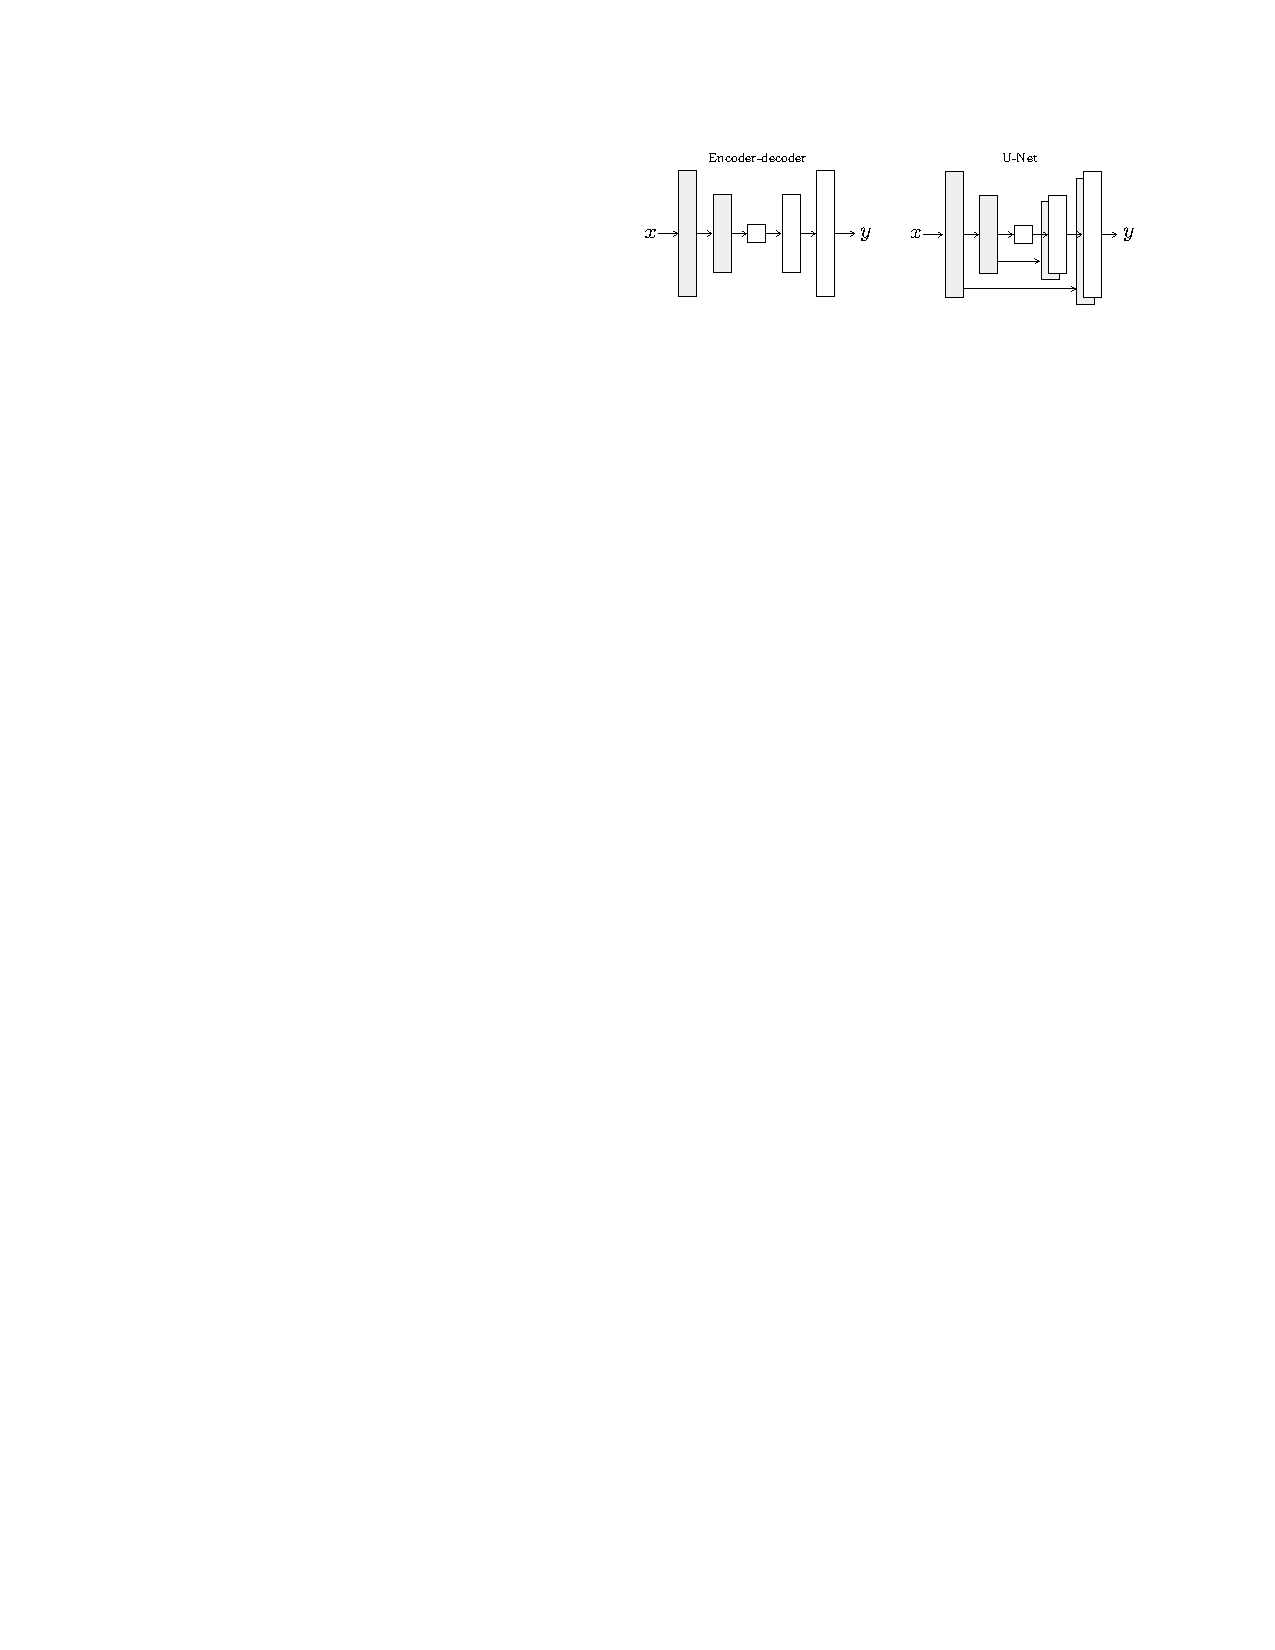
\includegraphics[width=0.7\textwidth]{../thesis/assets/pix2pix_unet.pdf}
\end{center}
\item Loss Function: PatchGAN + L1
\end{itemize}
\end{frame}



\begin{frame}{Background - CycleGAN (2017, Jun-Yan Zhu et al.)}
\vspace{-1em}
\begin{center}
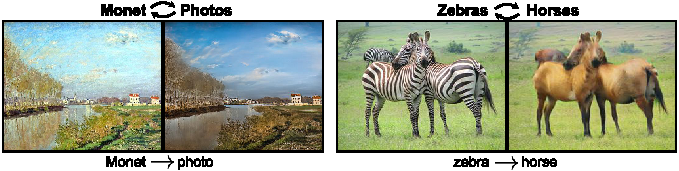
\includegraphics[width=0.95\textwidth]{assets/cyclegan_examples_small.pdf}
\end{center}
\vspace{-1em}
\textbf{Capabilities:}
\begin{itemize}
\item mapping between two visual representations
\end{itemize}
\textbf{Requirements:}
\begin{itemize}
\item one dataset of each domain \emph{without} pairwise annotation
\end{itemize}
\footfullcite{cyclegan}
\end{frame}





\begin{frame}{Skeletonization - Datasets}
\begin{columns}
\begin{column}{0.45\textwidth}

\includegraphics[width=\textwidth]{assets/cvl_vs_iam-online/cvl_0042-2-4_small.png}
\end{column}
\begin{column}{0.45\textwidth}
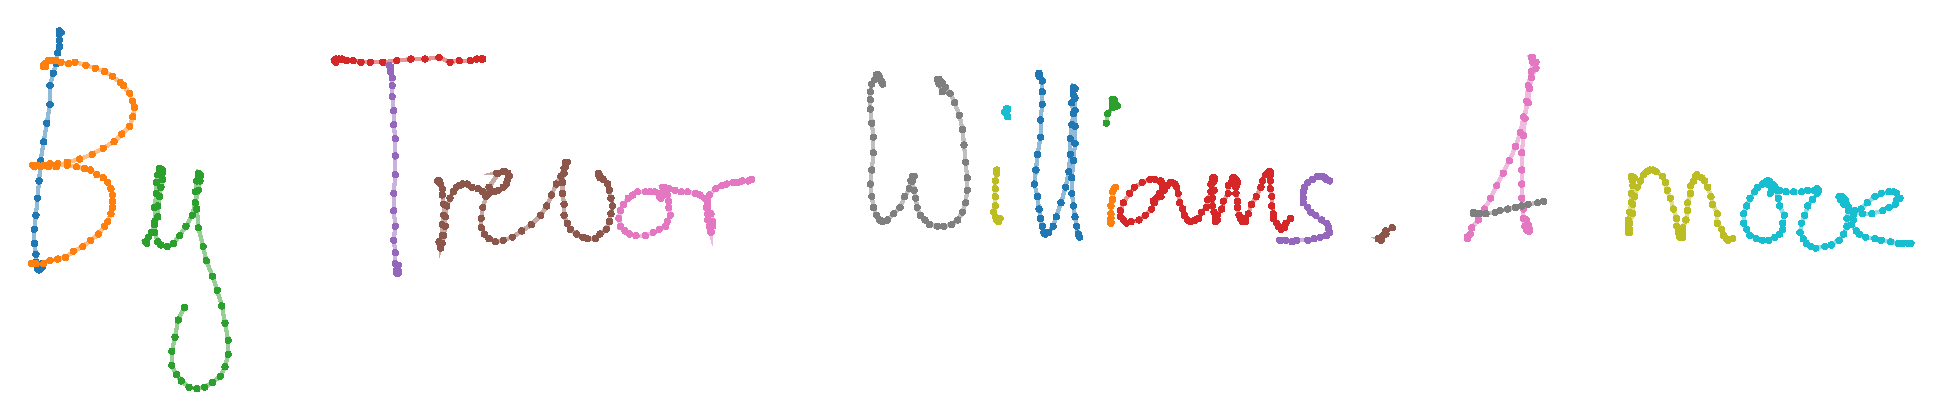
\includegraphics[width=\textwidth]{assets/cvl_vs_iam-online/iam-online.pdf}
\end{column}
\end{columns}
\vspace{1em}

\begin{columns}
\begin{column}{0.45\textwidth}
\textbf{CVL}
\begin{itemize}
\item Offline handwriting, white background
\item 310 writers
\item 7 texts (ca. 65 words per text)
\item ca. 15000 lines of text
\end{itemize}
\end{column}

\begin{column}{0.45\textwidth}
\textbf{IAM On-Line}
\begin{itemize}
\item Online handwriting
\item 221 writers
\item 1700 forms
\item 13049 lines of text
\end{itemize}
\end{column}
\end{columns}

\vspace{2em}
\textbf{But:} no pairwise annotations between them \footfullcite{cvl}\footfullcite{iam-online}
\vspace{1em}
\end{frame}


\begin{frame}{Skeletonization - First attempt: CycleGAN}
\vspace{-1em}
\begin{figure}[H]
\subfloat[skeleton]{
	
\includegraphics[width=0.3\textwidth]{../thesis/assets/skeletonization/cyclegan_fail/epoch004_real_A_crop.png}
    \hspace{1em}
}
\subfloat[synthetic image, produced by CycleGAN]{
    \hspace{1em}
  	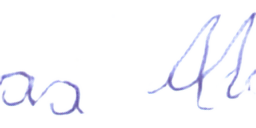
\includegraphics[width=0.3\textwidth]{../thesis/assets/skeletonization/cyclegan_fail/epoch004_fake_B_crop.png}
}
\end{figure}
\vspace{1em}
\textbf{Problems:}
\begin{itemize}
\item Datasets are created by different writers
\item CycleGAN adapts by changing the writer style
\end{itemize}
\end{frame}



\begin{frame}{Skeletonization - Second attempt: Pix2Pix}
\textbf{Problem:}
\begin{itemize}
\item No dataset with pairwise annotations available
\end{itemize}
\textbf{Solution:}
\begin{itemize}
\item Iterative knowledge transfer from a naive skeletonization
\end{itemize}
\begin{center}
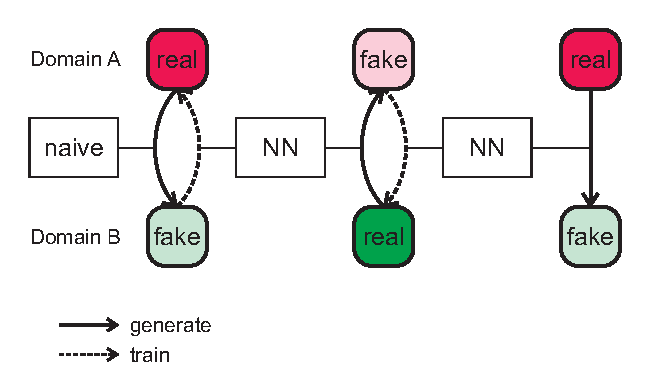
\includegraphics[width=0.5\textwidth]{assets/pix2pixTransfer.pdf}\hspace{5em}~
\end{center}
\end{frame}



\begin{frame}{Skeletonization - Second attempt: Pix2Pix}
\vspace{-1em}
\begin{figure}[H]
  \subfloat[CVL input data]{
  	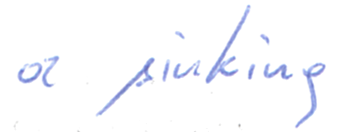
\includegraphics[width=0.32\textwidth]{../thesis/assets/skeletonization/comparison_pix2pix/0002-1-4_orig_crop.png}
  }
  \subfloat[primitive skeletonization]{
  	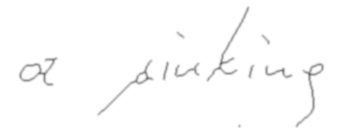
\includegraphics[width=0.32\textwidth]{../thesis/assets/skeletonization/comparison_pix2pix/0002-1-4_skel_prim_crop.png}
  }
  \subfloat[learned skeletonization]{
  	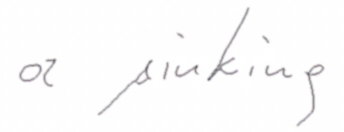
\includegraphics[width=0.32\textwidth]{../thesis/assets/skeletonization/comparison_pix2pix/0002-1-4_skel_nn_crop.png}
  }
\end{figure}
\vspace{1em}
\textbf{Improvements by knowledge transfer:}
\begin{itemize}
\item Less artifacts
\item Robustness towards contrast and brightness
\item Better handling of noise on the background
\end{itemize}
\end{frame}



\section{Stage 2: Conversion to Online Handwriting}
\begin{frame}{Conversion to Online Handwriting}
\begin{center}
\vspace{-1em}
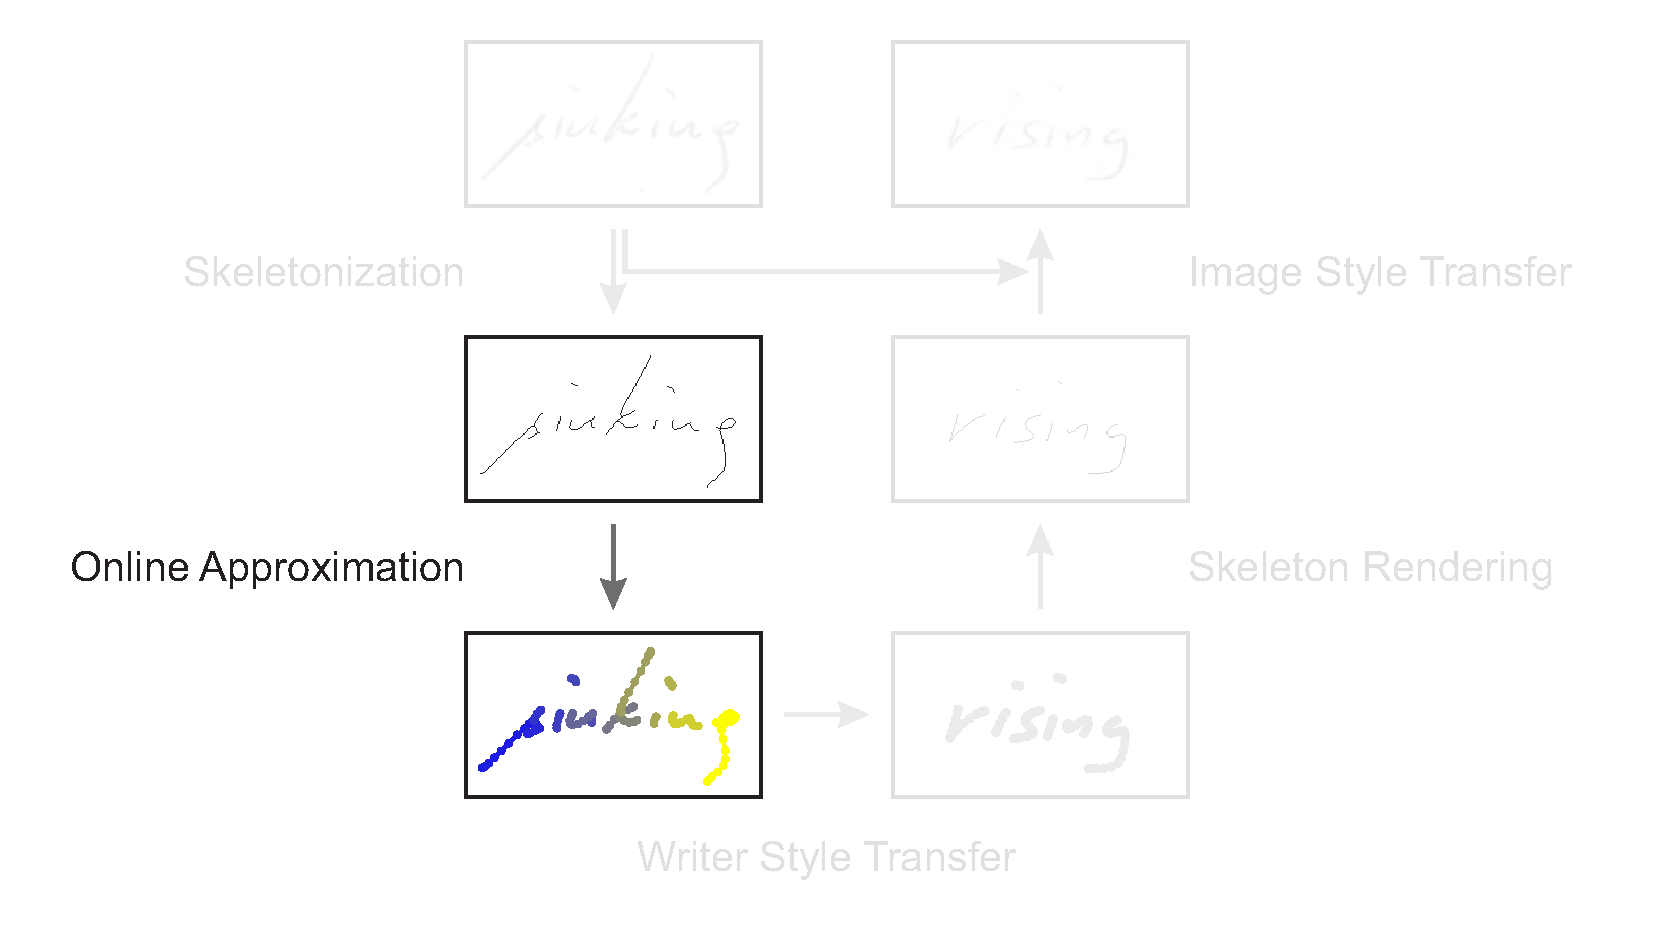
\includegraphics[width=0.85\textwidth]{assets/pipeline/pipeline_conversion.pdf}
\end{center}
\end{frame}



\begin{frame}{Graph Creation and Refinement}
\begin{center}
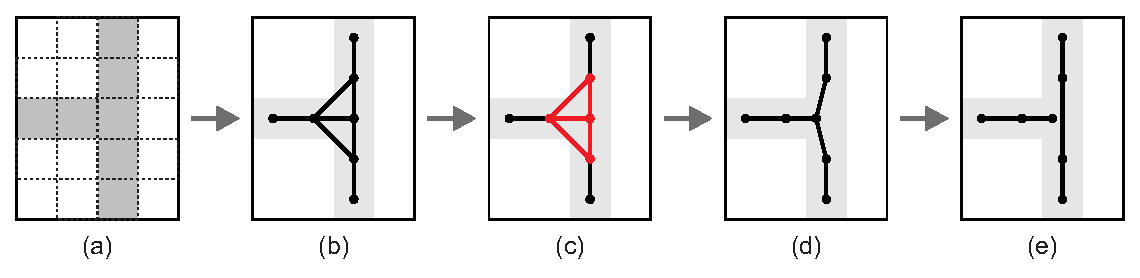
\includegraphics[width=0.85\textwidth]{../thesis/assets/sampling/cluster_removal/cluster_removal.pdf}
\end{center}
\textbf{Additional Steps} (not shown):
\begin{itemize}
\item Breaking of Cycles
\item Reordering
\end{itemize}
\end{frame}



\begin{frame}{Resampling}
\textbf{Reasons for resampling:}
\begin{itemize}
\item Less memory requirements
\item Closer to real handwriting
\item Better predictability in next stage
\end{itemize}
\vspace{1em}
\textbf{Methods:}
\begin{itemize}
\item \emph{Constant Velocity Resampling}
\begin{itemize}
\item Simple and easy to implement
\item Still unrealistic and restrictive
\end{itemize}
\item \emph{Maximum Acceleration Resampling}
\begin{itemize}
\item Closer to real handwriting, better understandable for predictions
\item More complex
\end{itemize}
\end{itemize}
\end{frame}



\begin{frame}{Maximum Acceleration Resampling}
\textbf{Algorithm:}
\begin{itemize}
\item Basic Principle is a \emph{4D Dijkstra Shortest Path Search}
\item Every node consists of:
\begin{itemize}
    \item $p_x$,$p_y$ - Point Coordinates
    \item $v_x$,$v_y$ - Incoming Velocity, defined as~ $\vec{v} = \vec{p} - \vec{p_{prev}}$
\end{itemize}
\item Velocities at first and last node are defined to be $\vec{0}$
\item Maximum acceleration constraint: $\norm{\vec{v} - \vec{v}_{prev}} < a$
\item Further constraint necessary to prevent shortcuts
\end{itemize}

\vspace{1em}
\textbf{Performance Optimizations:}
\begin{itemize}
\item Dynamic programming
\item Implementation in \emph{C}
\end{itemize}
\end{frame}




\begin{frame}{Resampling Comparison}
\begin{center}
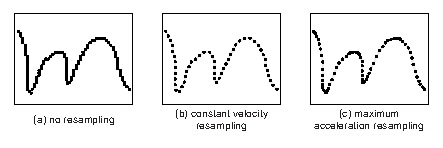
\includegraphics[width=0.99\textwidth]{../thesis/assets/sampling/sampling/resampling_comparison.pdf}

\end{center}
\end{frame}



\section{Stage 3: Writer Style Transfer}
\begin{frame}{Writer Style Transfer}
\begin{center}
\vspace{-1em}
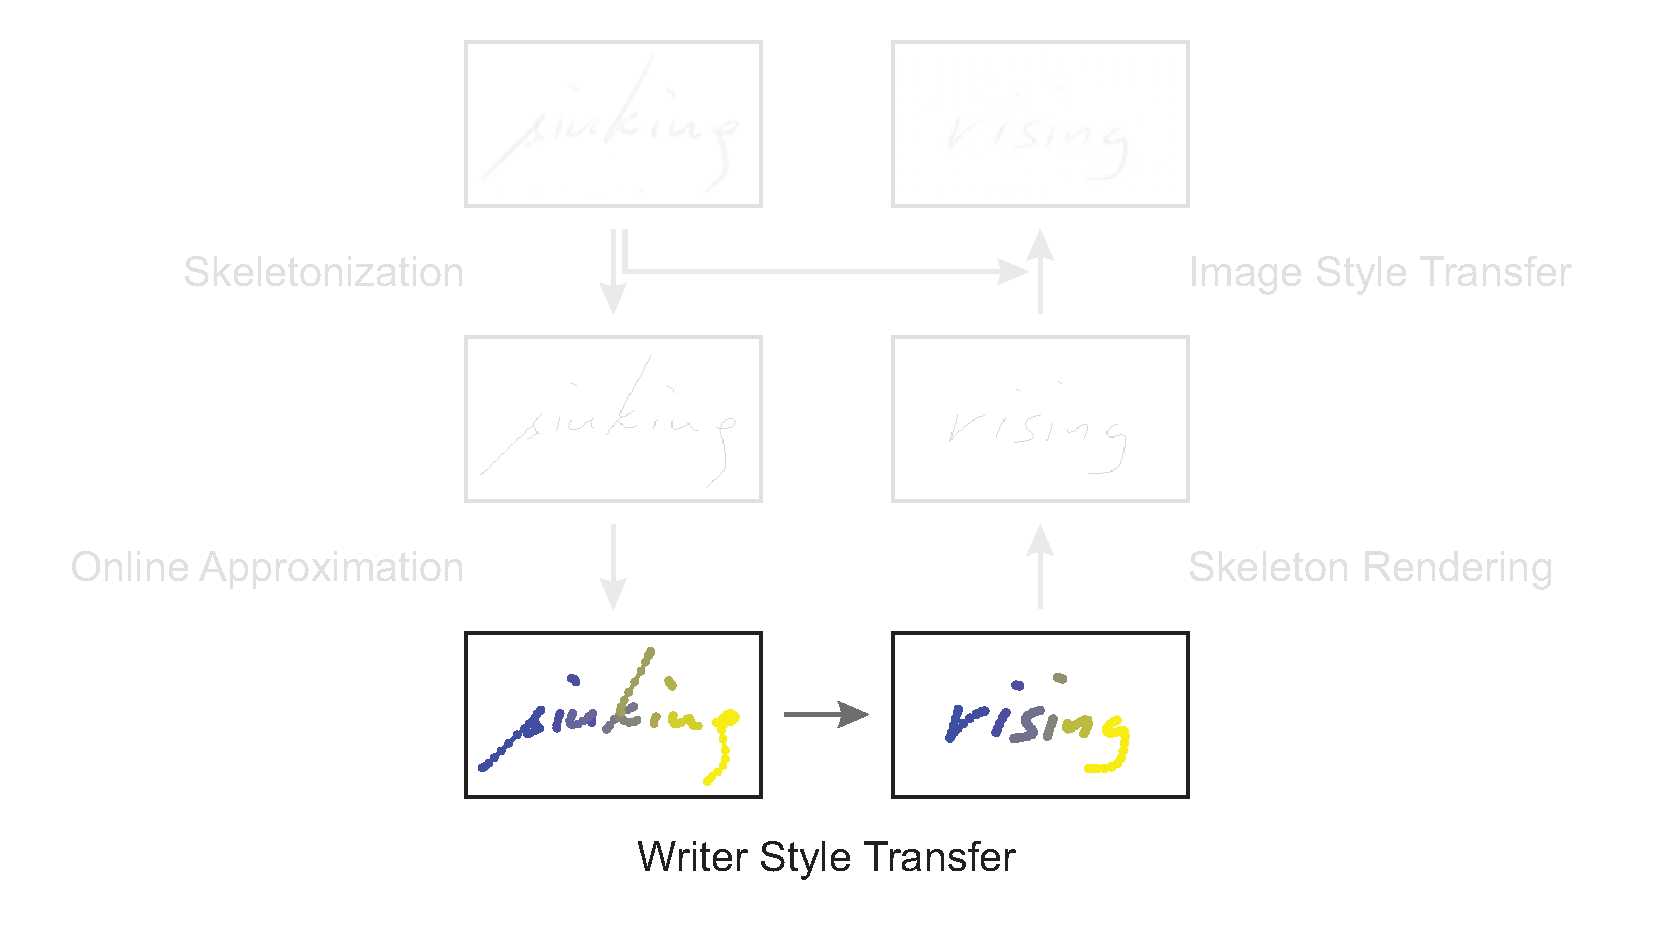
\includegraphics[width=0.85\textwidth]{assets/pipeline/pipeline_writerstyle.pdf}
\end{center}
\end{frame}




\begin{frame}{Writer Style Transfer}
\begin{itemize}
\item Has already been solved for real data
\item \emph{Challenge}: Extend to synthetic data
\end{itemize}
\vspace{1em}
\textbf{Algorithms:}
\begin{itemize}
\item Graves' Prediction Network
\item DeepWriting
\end{itemize}
\footfullcite{graves}
\footfullcite{deepwriting}
\end{frame}


\begin{frame}{Background: Graves' Network (2013, Alex Graves)}
\begin{columns}
\begin{column}{0.45\textwidth}
    \begin{itemize}
    \item Originally just a demonstration of \emph{LSTM} cell capabilities
    \item Works with online handwriting
    \item Predicts future pen position
    \item Takes the text content as additional input
    \item Attention mechanism to read the text content
    \end{itemize}
    \vspace{1em}
    \textbf{Handwriting Synthesis:}
    \begin{itemize}
    \item \emph{Prime} network with target style
    \item Continue with target content, feed predicted positions back into the network
    \end{itemize}
\end{column}
\begin{column}{0.50\textwidth}
    \begin{center}
    \vspace{-1em}
    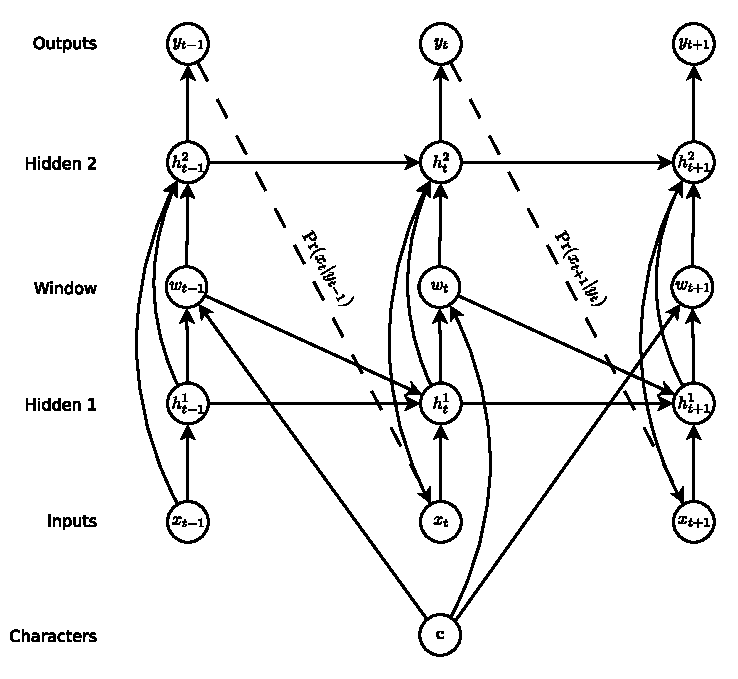
\includegraphics[width=0.95\textwidth]{../thesis/assets/style_transfer/graves_synthesis_network.pdf}
    \end{center}
\end{column}
\end{columns}
\end{frame}




\begin{frame}{Background: DeepWriting (2018, Emre Aksan et al.)}
\begin{itemize}
\item \emph{Conditional Variational Recurrent Neural Network}
\item Splits content and style into separate latent random variables
\end{itemize}

\vspace{1em}
\textbf{Advantages:}
\begin{itemize}
\item Style and content are stored explicitly
\end{itemize}

\vspace{1em}
\textbf{Disadvantages:}
\begin{itemize}
\item Requires \emph{EOC} and \emph{BOW} annotations
\item Only looks at one content character, switches at \emph{EOC}-signal\\$\Rightarrow$ No character look-ahead
\end{itemize}
\end{frame}




\begin{frame}{Writer Style Transfer: Experiments}
\begin{figure}[H]
  \vspace{-1em}
  \subfloat[Style Input]{
  	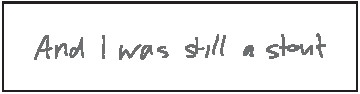
\includegraphics[width=0.34\textwidth]{assets/writer_transfer_results/comparison_style_input.pdf}
  }\\
  \pause
  \subfloat[DeepWriting + Constant Velocity]{
  	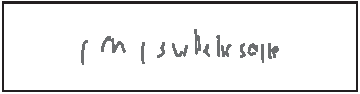
\includegraphics[width=0.34\textwidth]{assets/writer_transfer_results/comparison_deepwriting_velocity.pdf}
  }
  \hspace{1em}
  \pause
  \subfloat[DeepWriting + Maximum Acceleration]{
  	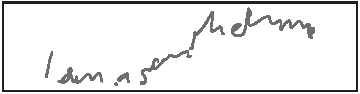
\includegraphics[width=0.34\textwidth]{assets/writer_transfer_results/comparison_deepwriting_acceleration.pdf}
  }\\
  \pause
  \subfloat[Graves + Maximum Acceleration]{
  	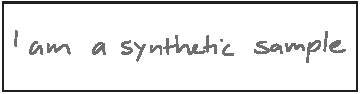
\includegraphics[width=0.34\textwidth]{assets/writer_transfer_results/comparison_graves_acceleration.pdf}
  }
\end{figure}
\end{frame}





\begin{frame}{Writer Style Transfer: Qualitative Demonstration}
\begin{table}
  \centering
  \resizebox{0.7\textwidth}{!}{
  \begin{tabular}{ll}
  \toprule
  Style Input & Output \\
  \midrule
  \raisebox{-0.4\height}{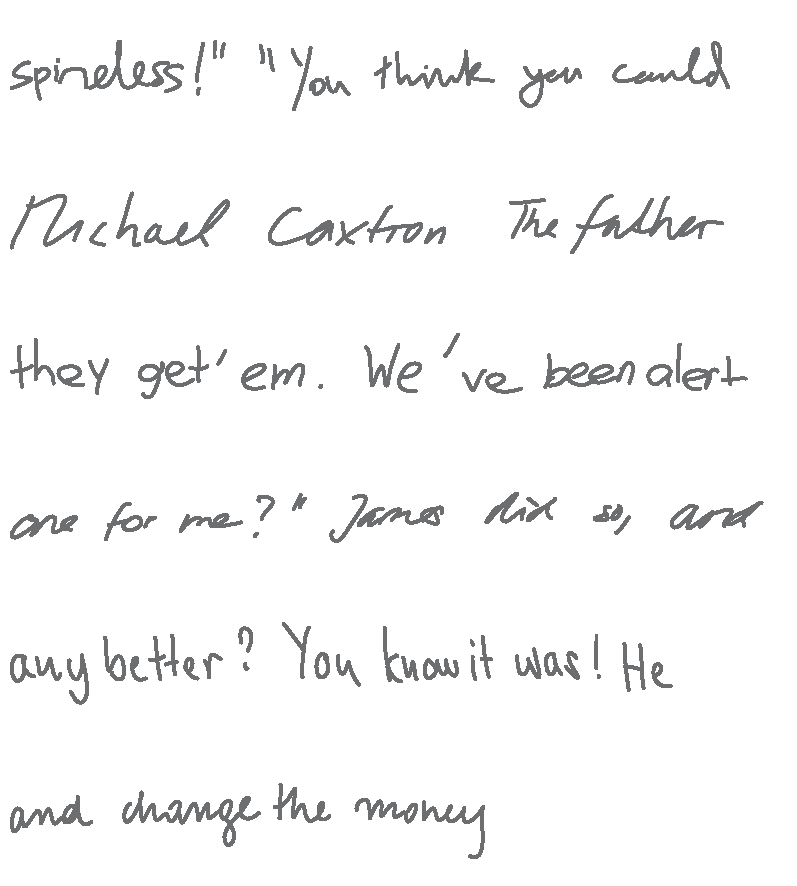
\includegraphics[scale=0.5]{../thesis/assets/style_transfer/style_transfer_in.pdf}} &
  \raisebox{-0.4\height}{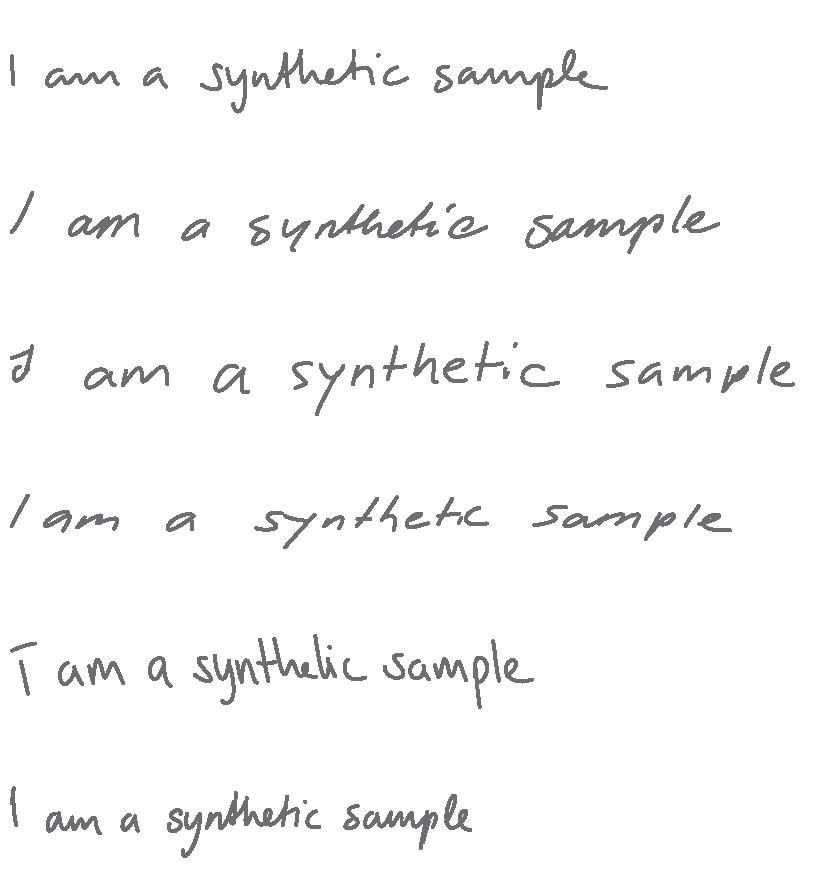
\includegraphics[scale=0.5]{../thesis/assets/style_transfer/style_transfer_out.pdf}} \\
  \bottomrule
  \end{tabular}
  }
\end{table}
\end{frame}





\section{Stage 4: Pen Style Transfer}
\begin{frame}{Pen Style Transfer}
\begin{center}
\vspace{-1em}
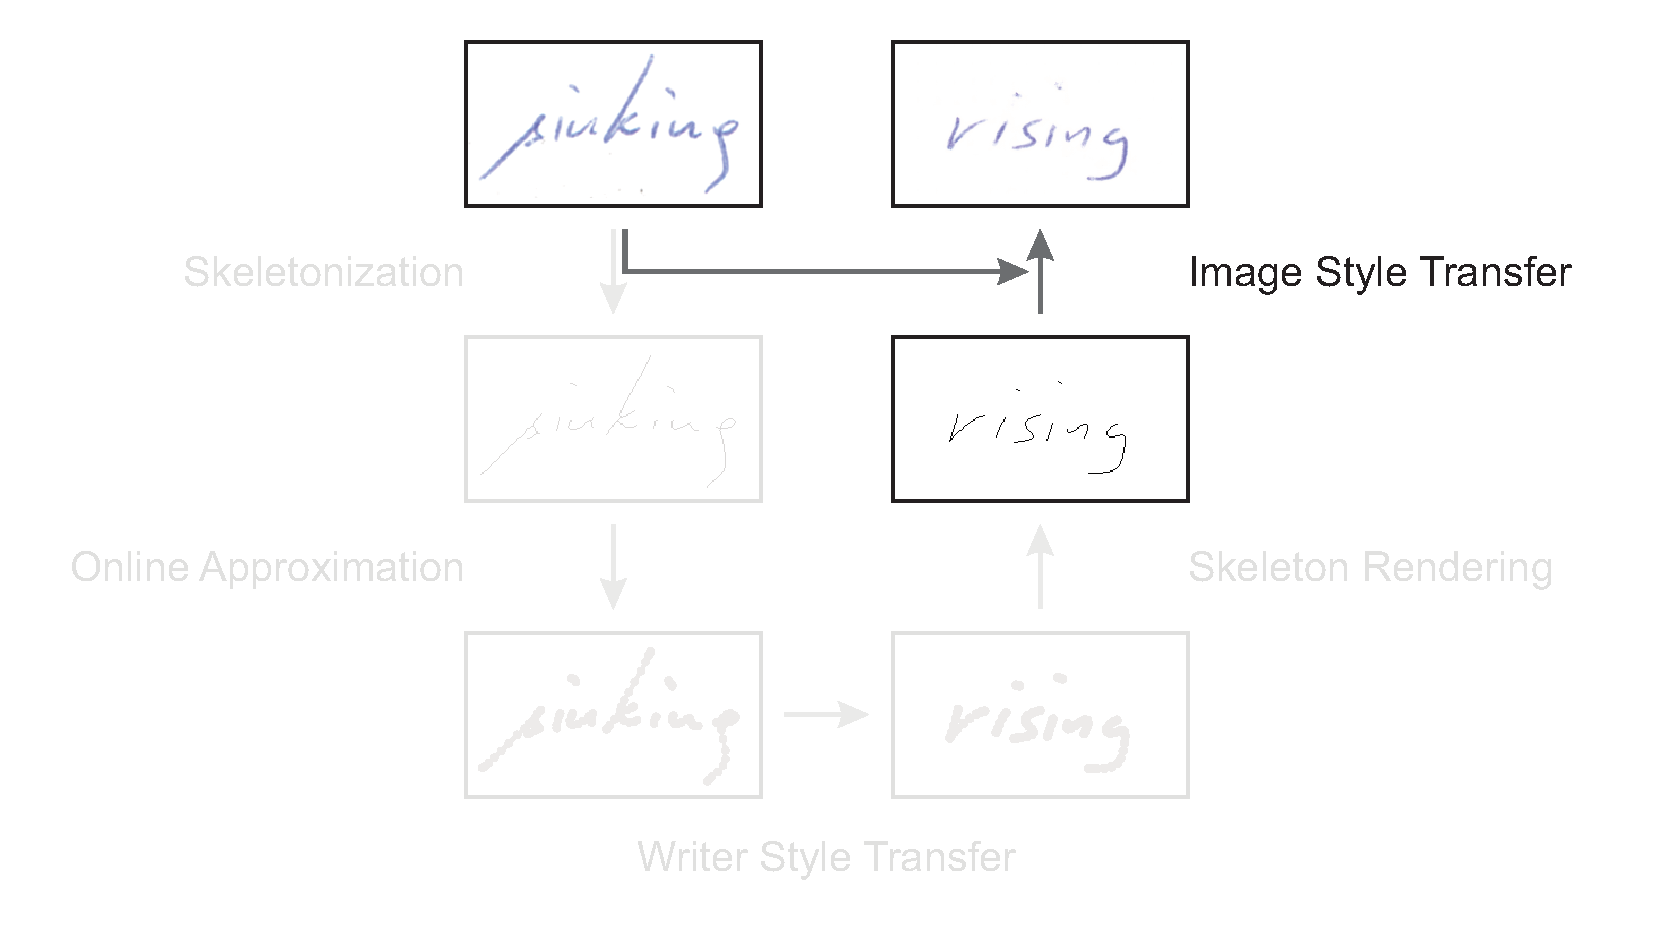
\includegraphics[width=0.85\textwidth]{assets/pipeline/pipeline_pentransfer.pdf}
\end{center}
\end{frame}




\begin{frame}{Pen Style Transfer}
Pix2Pix already proved to work (without style transfer)\\
$\Rightarrow$ promising, but modifications necessary

\vspace{1em}
\textbf{Modifications:}
\begin{itemize}
\item Style extraction network
\item Side input for Pix2Pix to inject style information
\item Changes in training procedure to encourage style transfer
\item (\emph{Not shown}: Fine-tuning of depth and feature sizes)
\end{itemize}
\end{frame}




\begin{frame}{Pen Style Transfer: Style Extraction}
\begin{center}
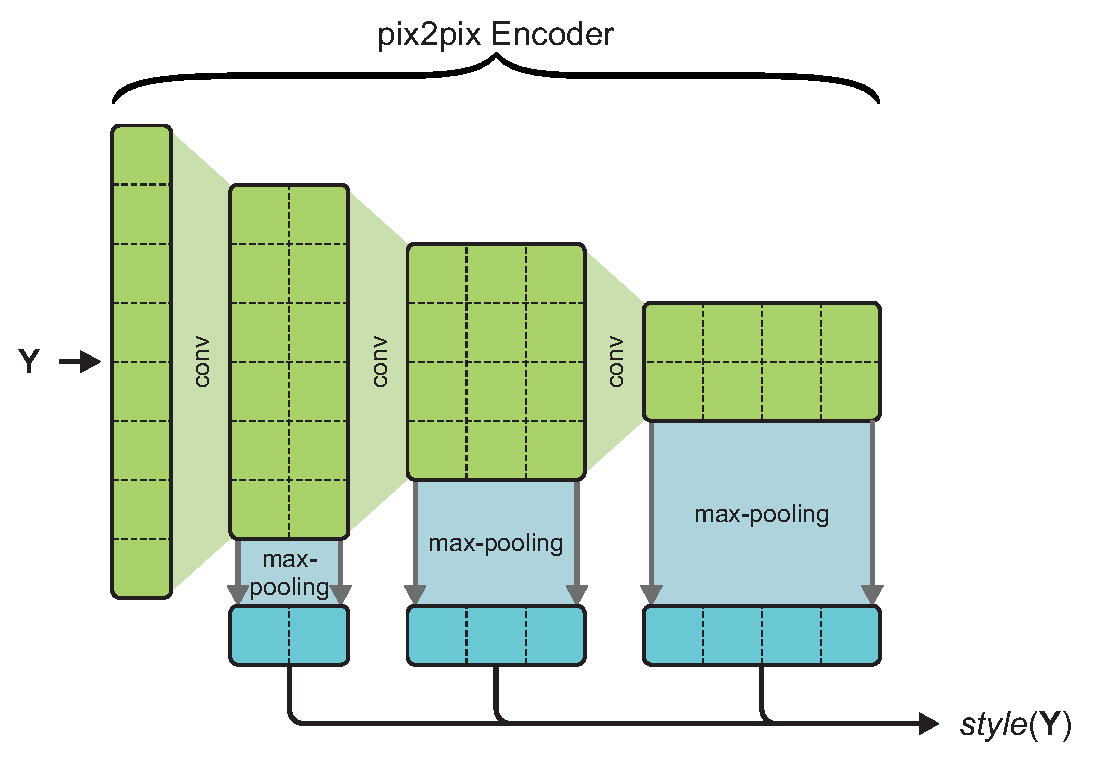
\includegraphics[width=0.60\textwidth]{../thesis/assets/pen_style_transfer/styleExtraction.pdf}
\end{center}  
\end{frame}



\begin{frame}{Pen Style Transfer: Style Injection into Generator Network}
\begin{center}
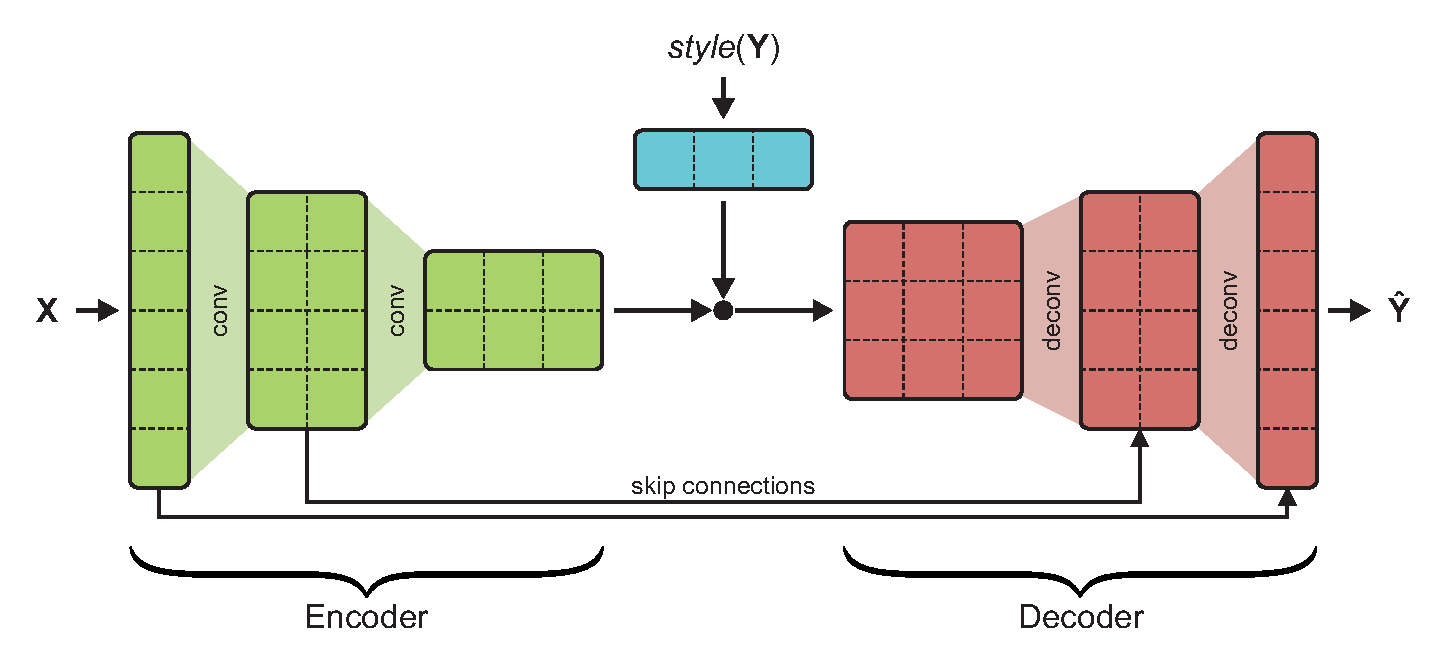
\includegraphics[width=0.80\textwidth]{../thesis/assets/pen_style_transfer/modifiedPix2Pix.pdf}
\end{center}  
\end{frame}



\begin{frame}{Pen Style Transfer: Conditional GAN Training}
\begin{center}
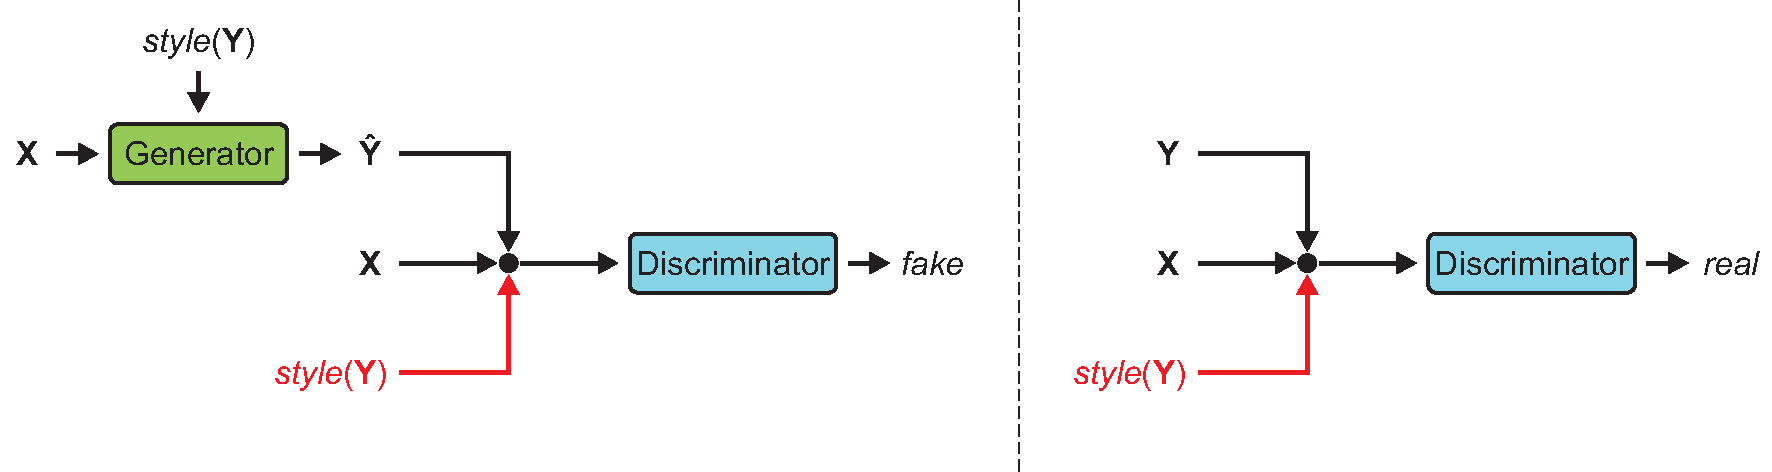
\includegraphics[width=0.95\textwidth]{assets/modifiedPix2PixTraining.pdf}
\end{center}  
\end{frame}



\begin{frame}{Pen Style Transfer: Results}
\begin{table}
  \centering
  \resizebox{0.51\textwidth}{!}{  
  \begin{tabular}{ll}
  \toprule
  Style Input & \hspace{.01\textwidth} Output \\
  \midrule
  \raisebox{-0.4\height}{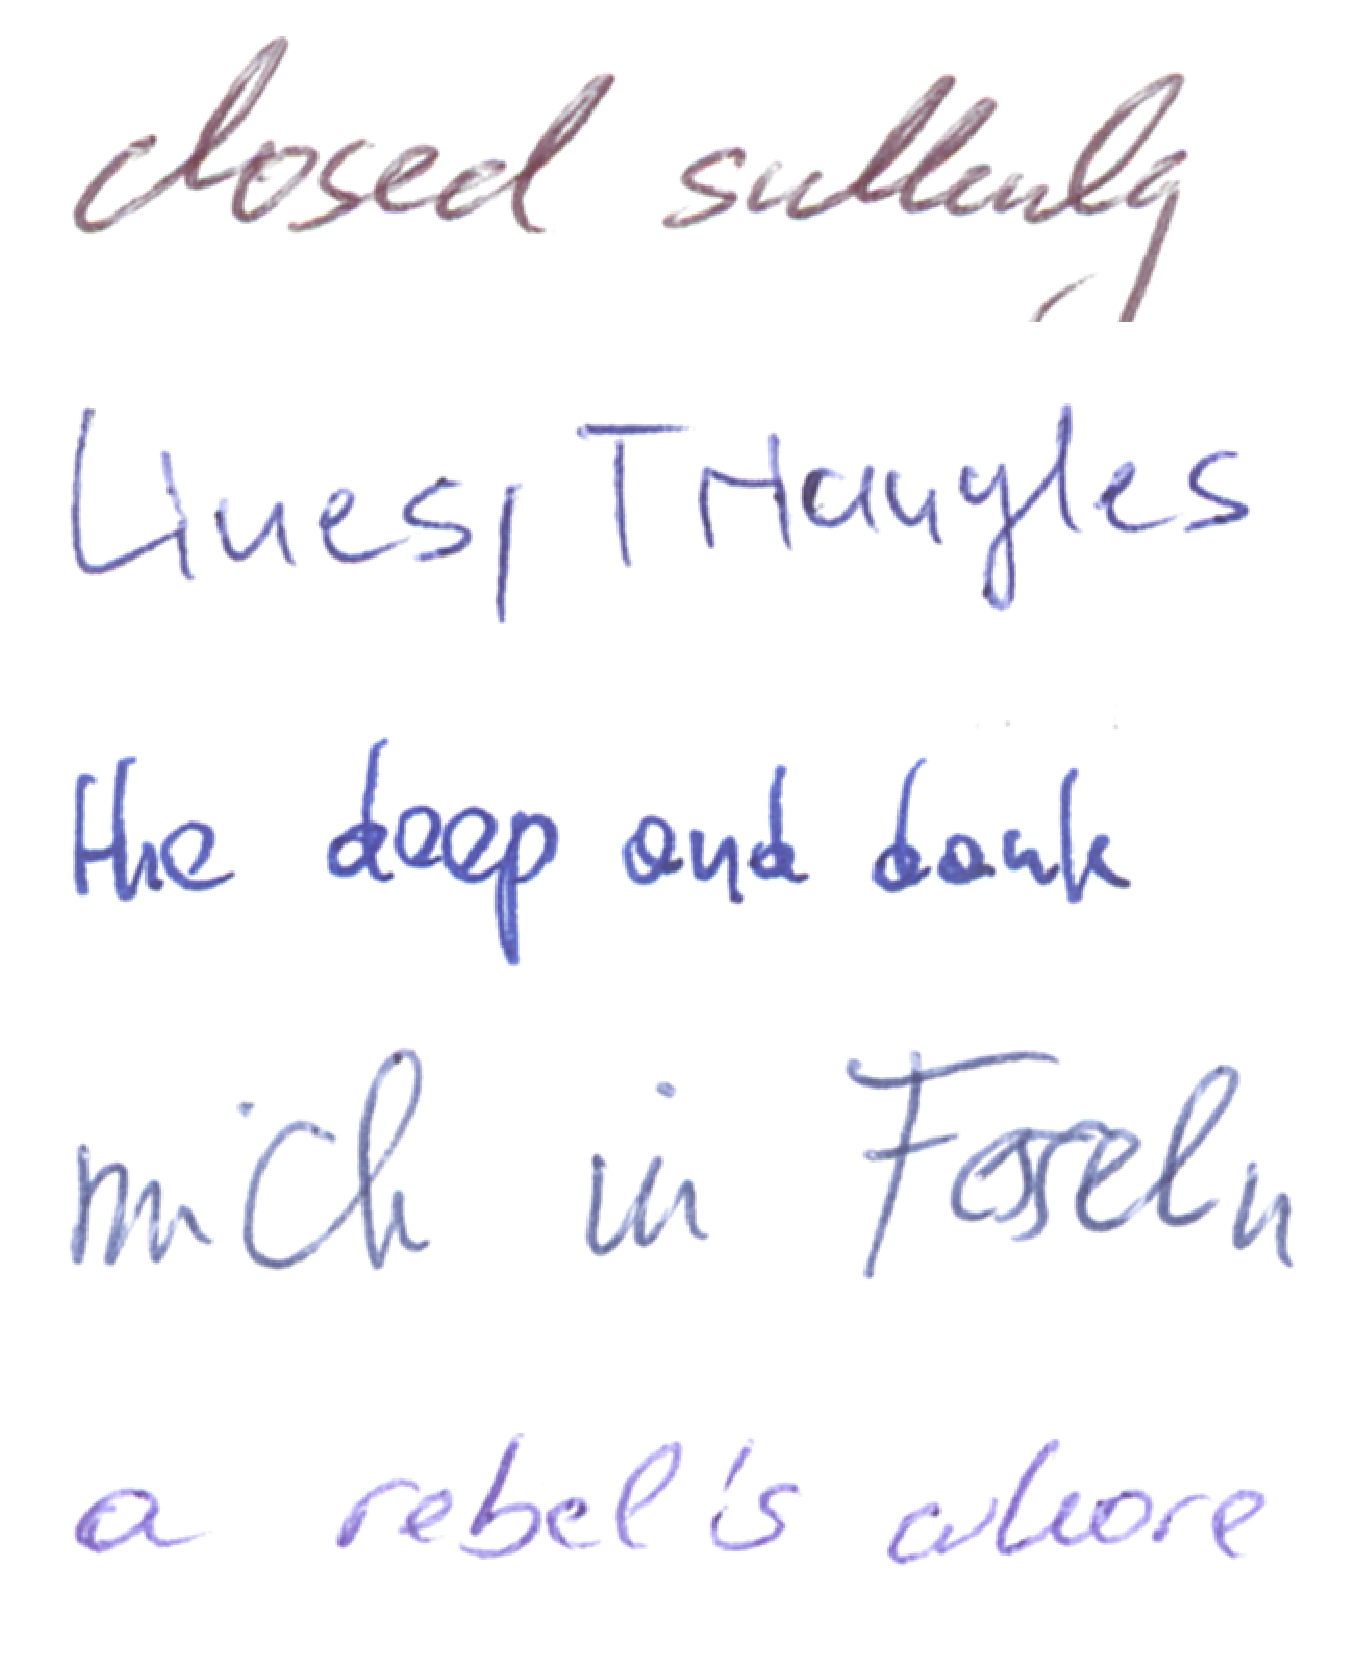
\includegraphics[scale=0.25]{../thesis/assets/pen_style_transfer/styles/style_demo_in.pdf}} &
  \raisebox{-0.4\height}{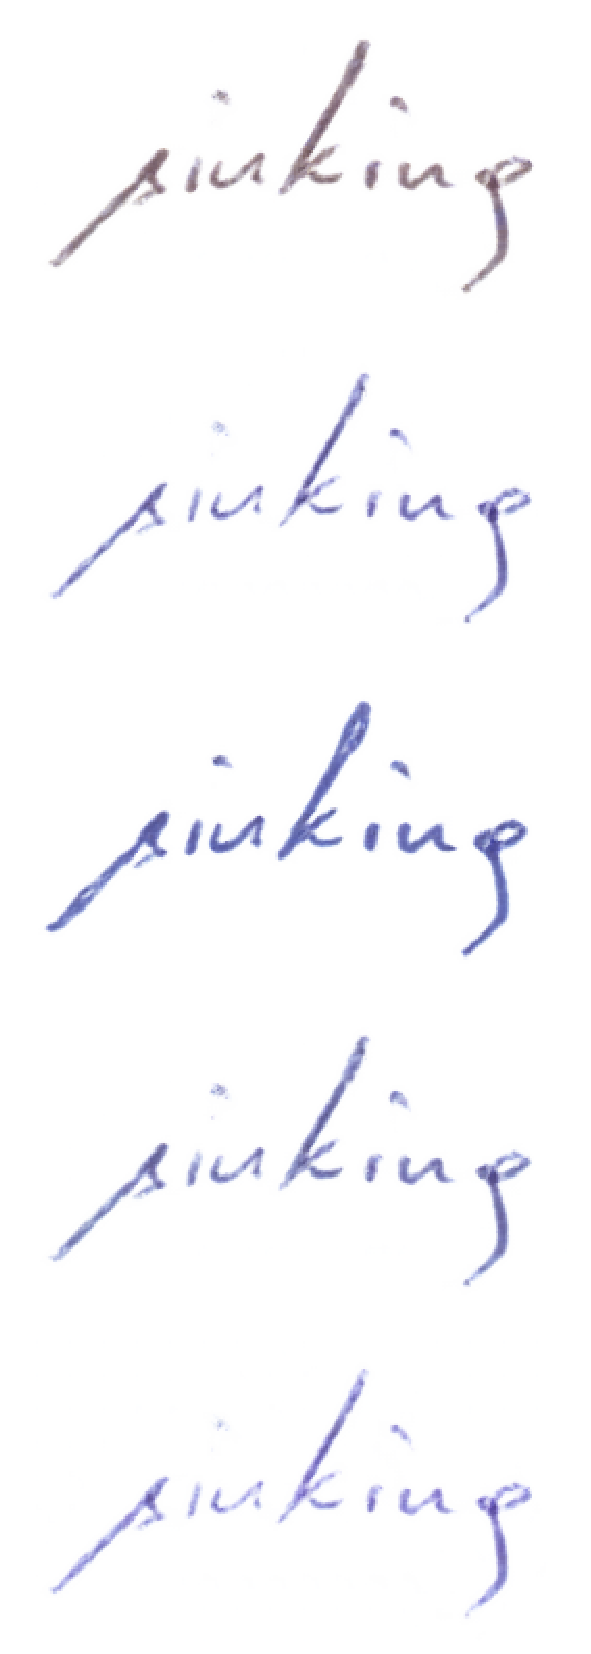
\includegraphics[scale=0.25]{../thesis/assets/pen_style_transfer/styles/style_demo_out.pdf}} \\
  \bottomrule
  \end{tabular}
  }
\end{table}
\end{frame}




\section{Conclusion \& Future Work}




\begin{frame}{Conclusion}
\textbf{Goals of this thesis:}
\begin{itemize}
\item Full offline-to-offline handwriting style transfer algorithm\\
\textcolor{red}{\hspace{1em}$\Rightarrow$ Success}
\item Finding a robust algorithm for handwriting skeletonization\\
\textcolor{red}{\hspace{1em}$\Rightarrow$ Success}
\item Is an offline to online handwriting conversion sufficient to use online algorithms?\\
\textcolor{red}{\hspace{1em}$\Rightarrow$ It is!}
\item Finding a way to transfer the pen style to the output image\\
\textcolor{red}{\hspace{1em}$\Rightarrow$ Success}
\item \emph{Optional:} Finding a way to transfer the background style to the output image\\
\textcolor{red}{\hspace{1em}$\Rightarrow$ Started, some success, but not shown here}
\end{itemize}
\end{frame}



\begin{frame}{Future Work}
\begin{itemize}
\item Further work on background style transfer
\item Combined skeletonization and sampling
\item Direct offline-to-offline style transfer
\end{itemize}
\end{frame}




\begin{frame}
\begin{center}
\begin{center}

\includegraphics[width=\textwidth]{assets/greetings/0047-4-3.png}\\

\includegraphics[width=\textwidth]{assets/greetings/0013-2-3.png}\\

\includegraphics[width=\textwidth]{assets/greetings/0042-2-4.png}
\end{center}
\end{center}
\end{frame}


















%% Appendix %%

\begin{frame}
\end{frame}


\begin{frame}{Appendix: Pix2Pix Knowledge Transfer Step 1}
\begin{figure}[H]
  \subfloat[real input image]{
  	\hspace{0.06\textwidth}
  	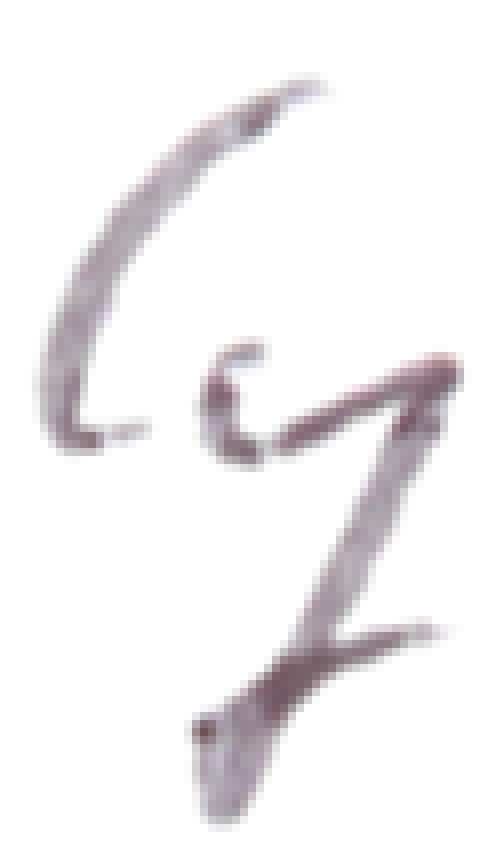
\includegraphics[width=0.15\textwidth]{../thesis/assets/skeletonization/net1_inverse/real_B_crop_large.png}
  	\hspace{0.06\textwidth}
  }
  \subfloat[primitive skeletonization]{
  \hspace{0.06\textwidth}
  	
\includegraphics[width=0.15\textwidth]{../thesis/assets/skeletonization/net1_inverse/real_A_crop_large.png}
  \hspace{0.06\textwidth}
  }
  \subfloat[trained network result]{
  	\hspace{0.06\textwidth}
  	
\includegraphics[width=0.15\textwidth]{../thesis/assets/skeletonization/net1_inverse/fake_B_crop_large.png}
  	\hspace{0.06\textwidth}
  }
\end{figure}
\end{frame}


\begin{frame}{Appendix: Pix2Pix Knowledge Transfer Step 2}
\begin{figure}[H]
  \subfloat[real skeleton]{
  	\hspace{0.05\textwidth}
  	
\includegraphics[width=0.19\textwidth]{../thesis/assets/skeletonization/net2_skeletonize/real_B_crop_large.png}
  	\hspace{0.05\textwidth}
  }
  \subfloat[synthetic image]{
  \hspace{0.05\textwidth}
  	
\includegraphics[width=0.19\textwidth]{../thesis/assets/skeletonization/net2_skeletonize/real_A_crop_large.png}
  \hspace{0.05\textwidth}
  }
  \subfloat[trained network result]{
  	\hspace{0.05\textwidth}
  	
\includegraphics[width=0.19\textwidth]{../thesis/assets/skeletonization/net2_skeletonize/fake_B_crop_large.png}
  	\hspace{0.05\textwidth}
  }
\end{figure}
\end{frame}


\begin{frame}{Appendix: Thresholding Hyperparameter Study}
  \centering
  \vspace{1em}
  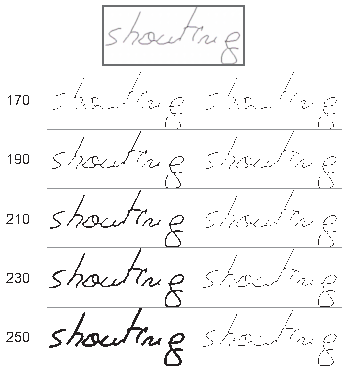
\includegraphics[width=0.4\textwidth]{../thesis/assets/skeletonization/thresholding_study/thresholding_study.pdf}
\end{frame}


\begin{frame}{Appendix: Skeletonization of Variable-Sized Images}
  \centering
  \vspace{1em}
  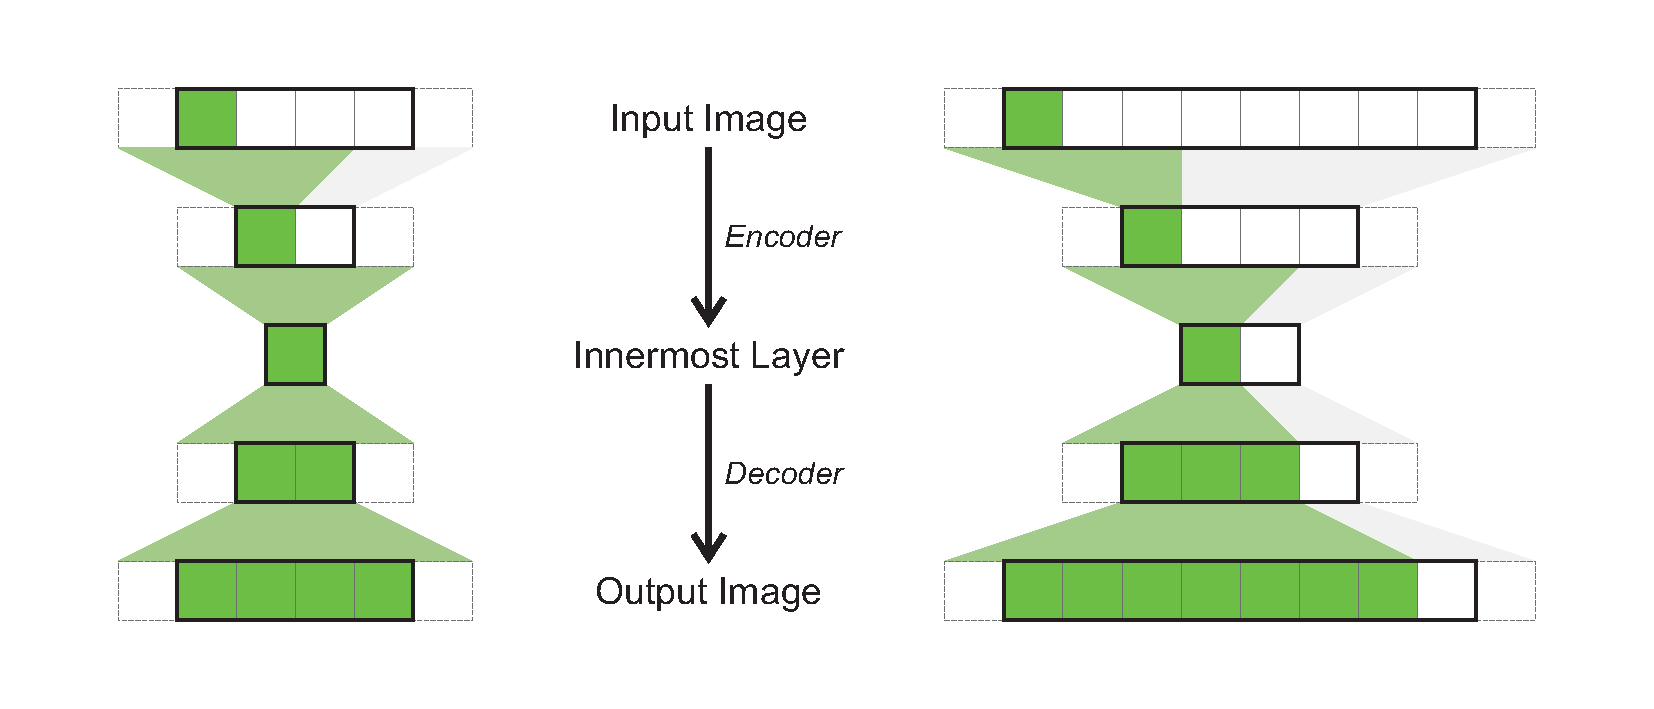
\includegraphics[width=0.9\textwidth]{../thesis/assets/pix2pixScaling.pdf}
\end{frame}

\begin{frame}{Appendix: Existing Problems with Skeletonizaton}
    \centering
    \vspace{1em}
    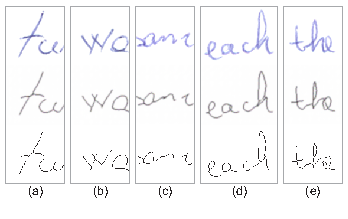
\includegraphics[width=0.75\textwidth]{../thesis/assets/skeletonization/compare_fail/fail_table.pdf}
\end{frame}

\begin{frame}{Appendix: Existing Problems with Online Conversion}
    \centering
    \vspace{1em}
    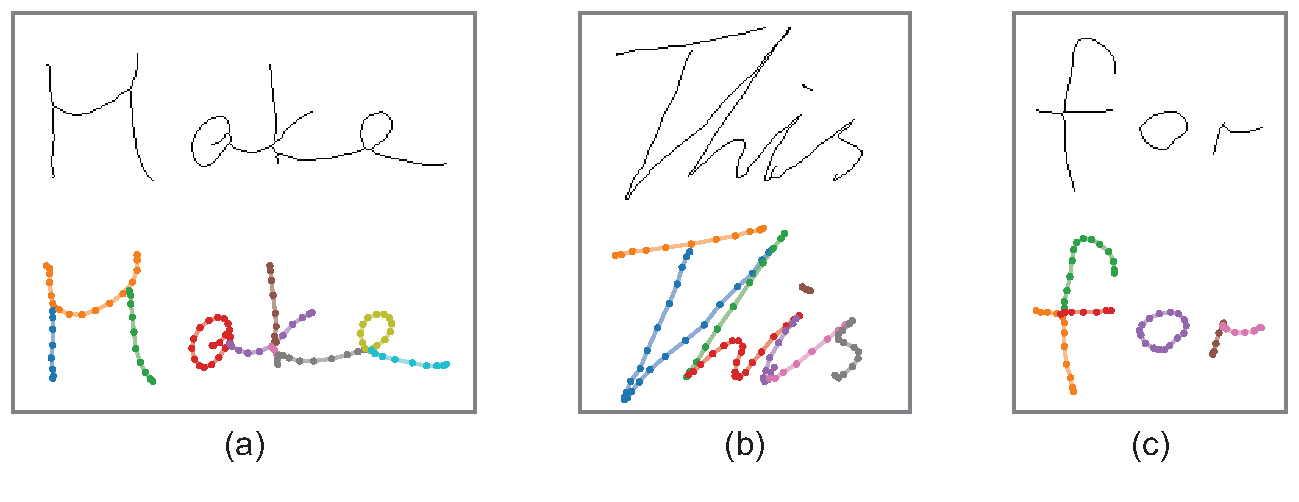
\includegraphics[width=0.90\textwidth]{../thesis/assets/sampling/fails/fails.pdf}
\end{frame}

\begin{frame}{Appendix: Existing Problems with the Online Conversion}
    \centering
    \vspace{1em}
    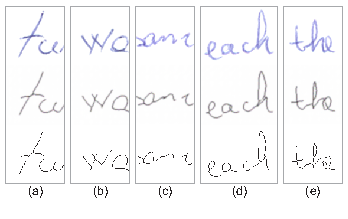
\includegraphics[width=0.75\textwidth]{../thesis/assets/skeletonization/compare_fail/fail_table.pdf}
\end{frame}


\begin{frame}{Appendix: Graves' Attention Window}
    \centering
    %\vspace{1em}
    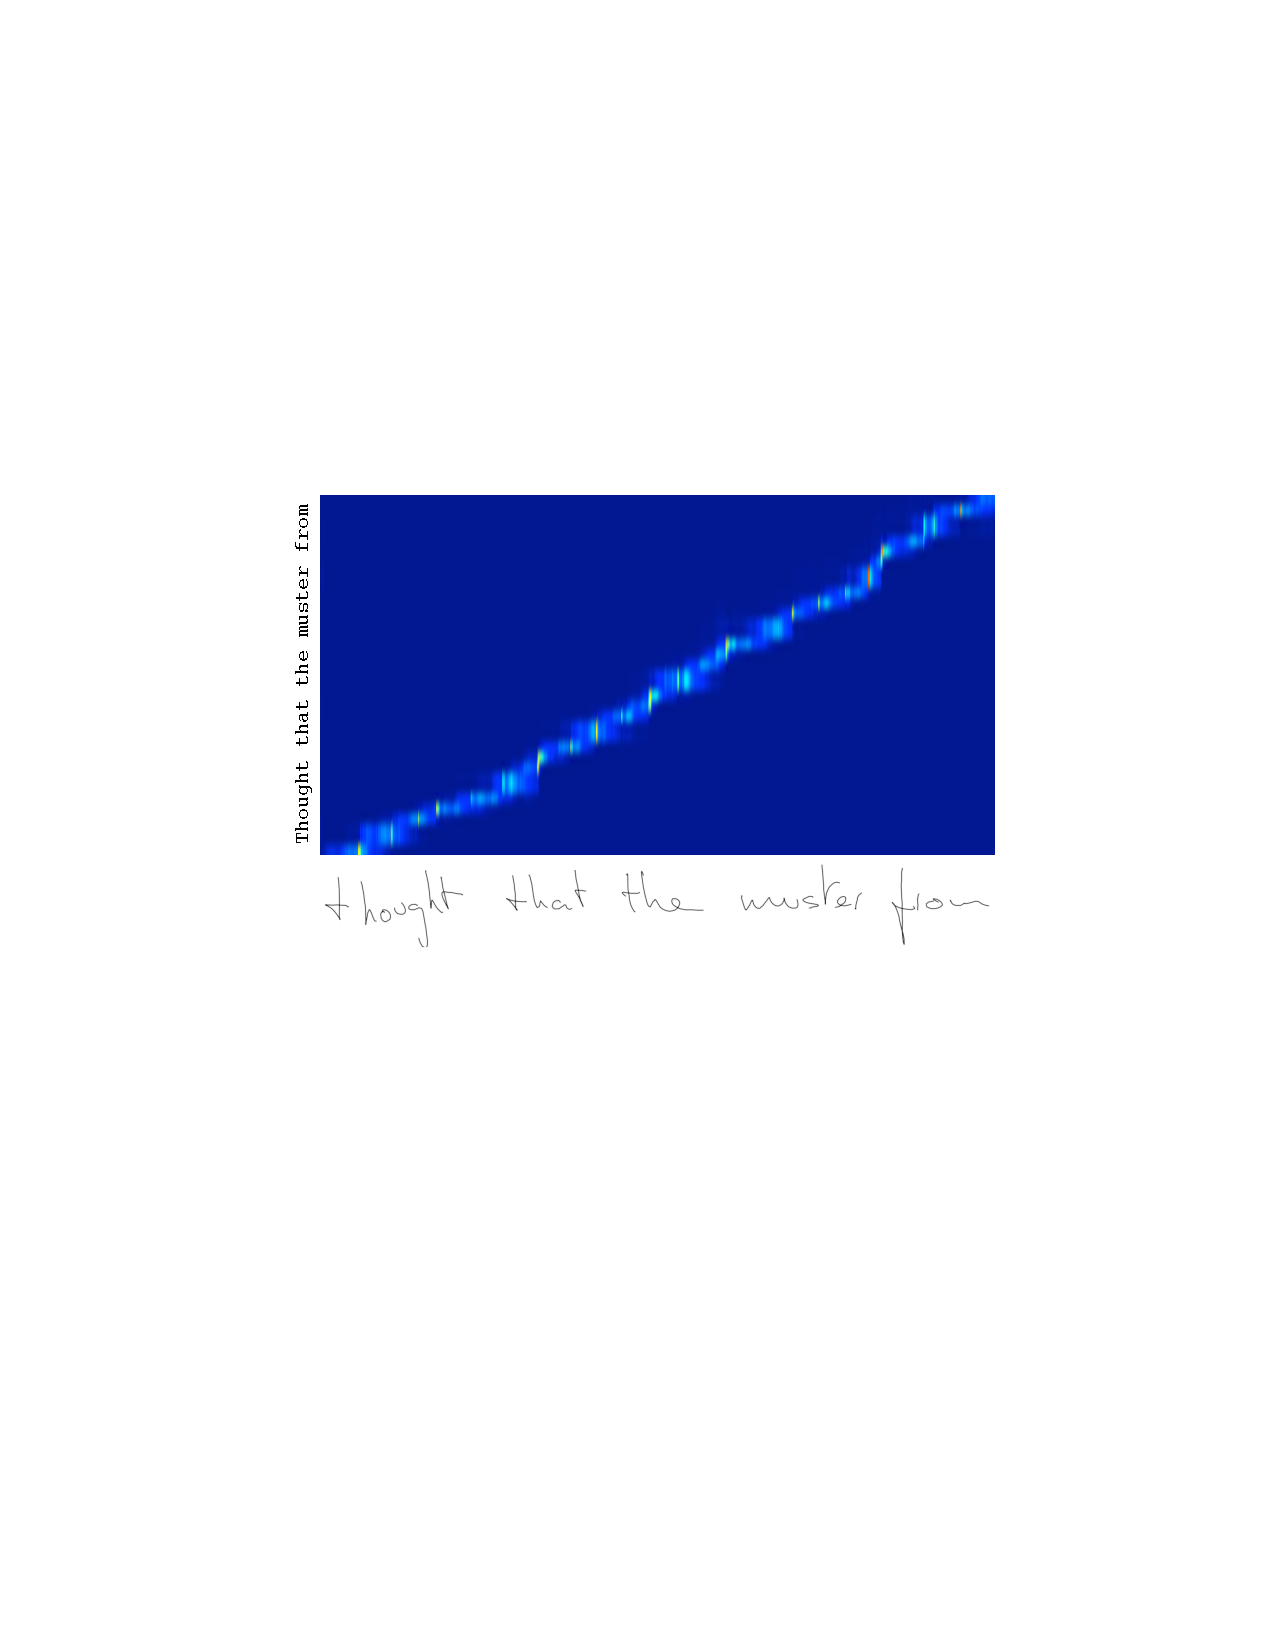
\includegraphics[width=0.65\textwidth]{../thesis/assets/style_transfer/graves_temporal_matching.pdf}
    \footfullcite{graves}
\end{frame}

\begin{frame}{Appendix: Existing Problems with Writer Style Transfer}
    \centering
    \vspace{1em}
    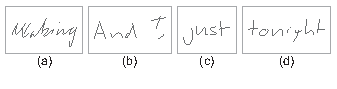
\includegraphics[width=0.75\textwidth]{../thesis/assets/style_transfer/failures.pdf}
\end{frame}


\begin{frame}{Appendix: Pen Style Transfer Error Correction Properties}
\begin{figure}[H]
  \centering
  \subfloat[skeleton input]{
  	
\includegraphics[width=0.25\textwidth]{../thesis/assets/pen_style_transfer/result_real_A.png}
  }
  \hspace{0.1\textwidth}
  \subfloat[network output]{
  	\includegraphics[width=0.25\textwidth]{../thesis/assets/pen_style_transfer/result_fake_B.png}
  }
\end{figure}
\end{frame}

\begin{frame}{Appendix: Background Style Transfer - Graves vs SPADE}
  \centering
  \vspace{1em}
  \resizebox{0.99\textwidth}{!}{  
  \begin{tabular}{lc}
  \toprule
  
  %Skeleton &
  %\raisebox{-0.45\height}{
  %\includegraphics[scale=0.18]{../assets/background_style_transfer/spade/skeleton_gray.png}%
  %}
  %\\
 % \midrule

  Style Input &  
 % \begin{varwidth}{1in}
  \raisebox{-0.45\height}{
  \includegraphics[scale=0.18]{../thesis/assets/background_style_transfer/spade/style/10.png}%
  \includegraphics[scale=0.18]{../thesis/assets/background_style_transfer/spade/style/38.png}%
  \includegraphics[scale=0.18]{../thesis/assets/background_style_transfer/spade/style/45.png}%
  \includegraphics[scale=0.18]{../thesis/assets/background_style_transfer/spade/style/46.png}%
  \includegraphics[scale=0.18]{../thesis/assets/background_style_transfer/spade/style/49.png}%
  \includegraphics[scale=0.18]{../thesis/assets/background_style_transfer/spade/style/31.png}%
  \includegraphics[scale=0.18]{../thesis/assets/background_style_transfer/spade/style/74.png}%
  \includegraphics[scale=0.18]{../thesis/assets/background_style_transfer/spade/style/99.png}%
 % \end{varwidth}%
  }
  \\%  
  Graves &
  %\begin{varwidth}{1in}
  \raisebox{-0.45\height}{
  \includegraphics[scale=0.18]{../thesis/assets/background_style_transfer/spade/result_pix2pix/10.png}%
  \includegraphics[scale=0.18]{../thesis/assets/background_style_transfer/spade/result_pix2pix/38.png}%
  \includegraphics[scale=0.18]{../thesis/assets/background_style_transfer/spade/result_pix2pix/45.png}%
  \includegraphics[scale=0.18]{../thesis/assets/background_style_transfer/spade/result_pix2pix/46.png}%
  \includegraphics[scale=0.18]{../thesis/assets/background_style_transfer/spade/result_pix2pix/49.png}%
  \includegraphics[scale=0.18]{../thesis/assets/background_style_transfer/spade/result_pix2pix/31.png}%
  \includegraphics[scale=0.18]{../thesis/assets/background_style_transfer/spade/result_pix2pix/74.png}%
  \includegraphics[scale=0.18]{../thesis/assets/background_style_transfer/spade/result_pix2pix/99.png}%
  }
  \\%  
  SPADE &
  %\begin{varwidth}{1in}
  \raisebox{-0.45\height}{
  \includegraphics[scale=0.18]{../thesis/assets/background_style_transfer/spade/result/10.png}%
  \includegraphics[scale=0.18]{../thesis/assets/background_style_transfer/spade/result/38.png}%
  \includegraphics[scale=0.18]{../thesis/assets/background_style_transfer/spade/result/45.png}%
  \includegraphics[scale=0.18]{../thesis/assets/background_style_transfer/spade/result/46.png}%
  \includegraphics[scale=0.18]{../thesis/assets/background_style_transfer/spade/result/49.png}%
  \includegraphics[scale=0.18]{../thesis/assets/background_style_transfer/spade/result/31.png}%
  \includegraphics[scale=0.18]{../thesis/assets/background_style_transfer/spade/result/74.png}%
  \includegraphics[scale=0.18]{../thesis/assets/background_style_transfer/spade/result/99.png}%
  }
  \\
  \bottomrule
  \end{tabular}
  }
  \footfullcite{graves}
  \footfullcite{spade}
\end{frame}


\begin{frame}{Appendix: Background Style Transfer - Pipeline}
    \centering
    \vspace{1em}
    \includegraphics[width=0.95\textwidth]{../thesis/assets/background_style_transfer/pipeline/pipeline.pdf}
\end{frame}





%%% REMOVED SLIDES %%%



\begin{frame}{Motivation}
\emph{Why?}
\begin{itemize}
\item Combining benefits of digital and handwritten text
\item Automated handwriting generation
\item Because we can
\item Getting new insights into neural networks
\end{itemize}
\end{frame}


\begin{frame}{Background - CycleGAN (2017, Jun-Yan Zhu et al.)}
\textbf{Cycle Consistency Training}
\vspace{-1em}
\begin{overprint}
\onslide<1>\centering\includegraphics[width=0.6\textwidth]{assets/cycleGanLoss_1.pdf}\hspace{5em}~
\onslide<2>\centering\includegraphics[width=0.6\textwidth]{assets/cycleGanLoss_2.pdf}\hspace{5em}~
\onslide<3>\centering\includegraphics[width=0.6\textwidth]{../thesis/assets/cycleGanLoss.pdf}\hspace{5em}~
\end{overprint}
\end{frame}


\begin{frame}{Writer Style Transfer: Training Data}
\textbf{Question:}
\begin{itemize}
\item What should the network be trained with?
\end{itemize}

\vspace{1em}
\textbf{Options:}
\begin{itemize}
\item \emph{Real Skeletons}:
\begin{itemize}
\item Contain less artifacts
\item Different from what it will see in the final pipeline
\item \textbf{Disadvantage}: Network might have trouble with style extraction
\end{itemize}

\item \emph{Synthetic Skeletons}:
\begin{itemize}
\item Contain more artifacts
\item Match what it will see in the final pipeline
\item \textbf{Disadvantage}: Network might produce more artifacts
\end{itemize}
\end{itemize}

\end{frame}




\begin{frame}{Writer Style Transfer: Training Data}
\begin{table}
  \centering
  \resizebox{0.9\textwidth}{!}{
  \begin{tabular}{lll}
  \toprule
  Training Data & Style Input & Result \\
  \midrule
  synthetic & synthetic & \raisebox{-0.4\height}{\includegraphics[scale=1.2]{../thesis/assets/style_transfer/real_synthetic_comparison/trained_reskeletonized_style_reskeletonized/synthetic_sample_lalign.pdf}} \\
  synthetic & real & \raisebox{-0.4\height}{\includegraphics[scale=1.2]{../thesis/assets/style_transfer/real_synthetic_comparison/trained_reskeletonized_style_online/synthetic_sample_lalign.pdf}} \\
  real & synthetic & \raisebox{-0.4\height}{\includegraphics[scale=1.2]{../thesis/assets/style_transfer/real_synthetic_comparison/trained_online_style_reskeletonized/synthetic_sample_lalign.pdf}} \\
  real & real & \raisebox{-0.4\height}{\includegraphics[scale=1.2]{../thesis/assets/style_transfer/real_synthetic_comparison/trained_online_style_online/synthetic_sample_lalign.pdf}} \\
  \midrule
  \multicolumn{2}{l}{Reference Style} & \raisebox{-0.4\height}{\includegraphics[scale=1.2]{../thesis/assets/style_transfer/real_synthetic_comparison/style.pdf}} \\
  \bottomrule
  \end{tabular}
  }
\end{table}
\end{frame}




\printbibliography

\end{document}
